\documentclass[a4paper, 12pt, oneside]{book}
\usepackage[left=2.5cm,right=2.5cm,top=2.5cm,bottom=2.5cm]{geometry}
\usepackage[spanish, es-noshorthands,activeacute]{babel} % es-noshorthands es para que no tenga problemas con tikz
\usepackage[latin1]{inputenc}
\usepackage{graphicx}
\usepackage{amssymb}
\usepackage{amsthm}
\usepackage{amsmath}
\usepackage{makeidx}
\usepackage{color}
\usepackage{algpseudocode}
\usepackage{hyperref}

\hyphenation{Polyno-mialtime}
%%%%%%%%%%%%%%%%%%%%%%%%%%%%%%%%%%%%%%%%%%%%%%%%%%%%%%%%%%%%%%%%%%%%
\newtheorem{definicion}{Definici\'on}[chapter]
\newtheorem{lema}{Lema}[chapter]
\newtheorem{proposicion}{Proposici\'on}[chapter]
\newtheorem{teorema}{Teorema}[chapter]
\newtheorem{corolario}{Corolario}[chapter]
\newtheorem{observacion}{Observaci\'on}[chapter]
\newtheorem{ejemplo}{Ejemplo}[chapter]
\newtheorem{ejercicio}{Ejercicio}[chapter]
%añadir [chapter] al final de cada comando si se desea que la numeración vaya acorde al capítulo

%%%%%%%%%%%%%%%%%%%%%%%%%%%%%%%%%%%%%%%%%%%%%%%%%%%%%%%%%%%%%%%%%%%%%
\renewcommand{\thesection}{\arabic{section}}
%%%%%%%%%%%%%%%%%%%%%%%%%%%%%%%%%%%%%%%%%%%%%%%%%%%%%%%%%%%%%%%%%%%%%




\begin{document}
	\pagenumbering{roman}
	%-------------------------------------------------------------------------Inicio P\'{a}gina del T\'{\i}tulo
	\begin{titlepage}
		
		
\includegraphics[scale=0.18]{logo-facultad-ciencias-uma}
		
		\vskip2truecm
		
		\begin{center}
			
			% Upper part of the page. The '~' is needed because \\
			% only works if a paragraph has started.
			
			%\includegraphics[width=0.35\textwidth]{\textbf{logo-facultad-ciencias-uma}}~\\[1cm]
			
			
			%\textsc{\LARGE Universidad de M\'{a}laga}
			
			%\textsc{Facultad de ciencias}\\ [1.5cm]
			
			%\textsc{\Large Trabajo Fin de Grado}\\[0.5cm]
			
			% Title
			%\noindent\rule{\textwidth}{0.4mm}
			{ \huge \bfseries Algoritmos para la resoluci\'on del problema combinatorio de empaquetamiento  \\[0.4cm] }
			
			%\noindent\rule{\textwidth}{0.4mm}
			\vskip1truecm
			
			{ \huge \bfseries Algorithms for the resolution of Bin Packing Problem \\[0.4cm] }
			
			%\noindent\rule{\textwidth}{0.4mm}
			
			
			\vskip1truecm
			
			{\Large Trabajo Fin de Grado en Matem\'aticas} \\
			
			{\Large Universidad de M\'alaga} \\
			
			%\vfill
		\end{center}
		
		\vskip2truecm
		
		\noindent\rule{\textwidth}{0.4mm}
		
		\vskip.2truecm
		
		
		{\bf Autor:} {Rafael Requena Garrido}\\
		
		{\bf \'{A}rea de conocimiento y/o departamento:} {Lenguajes y Sistemas Inform\'aticos} \\
		
		{\bf Fecha de presentaci\'{o}n:} {Septiembre de 2021}\\
		
		{\bf Tema:} {Resoluci\'on de problemas de optimizaci\'on combinatoria}\\
		
		{\bf Tipo:} {(trabajo de revisi\'on bibliogr\'afica, de iniciaci\'on a la investigaci\'on,...)}\\
		
		{\bf Modalidad:} {Individual}\\
		
		{\bf N\'umero de p\'aginas (sin incluir introducci\'on, bibliograf\'{\i}a ni anexos):}\\
		
		
		
		
	\end{titlepage}
	%-------------------------------------------------------------------------Fin P\'{a}gina del T\'{\i}tulo
	%----------------P\'agina en blanco--------------------------------------------------------------
	\newpage
	\mbox{}
	\thispagestyle{empty}
	%----------------Fin p\'agina en blanco---------------------------------------------------
	\begin{titlepage}
		\begin{center}
			
			
			
			\textsc{\Large DECLARACI\'{O}N DE ORIGINALIDAD DEL TFG}\\[0.5cm]
			\bigskip
			
			%\noindent\rule{\textwidth}{0.4mm}
			\vskip2truecm
			% Author and tutor
			%\begin{minipage}{0.4\textwidth}
			%\begin{flushleft} \large
			%\emph{Autor:}\\
			%\textsc{Nombre y Apellidos del autor}
			%\end{flushleft}
			%\end{minipage}
		\end{center}
		
		D./D\~{n}a. \textit{Rafael Requena Garrido}, con DNI (NIE o pasaporte) \textit{76437428X}, estudiante del Grado en \textit{Matem\'aticas} de la Facultad de Ciencias de la Universidad de M\'{a}laga,\\
		\textbf{DECLARO:}\\
		
		Que he realizado el Trabajo Fin de Grado titulado ``\textit{Algoritmos para la resoluci\'on del problema combinatorio de empaquetamiento}'' y que lo presento para su evaluaci\'{o}n. Dicho trabajo es original y todas las fuentes bibliogr\'{a}ficas utilizadas para su realizaci\'{o}n han sido debidamente citadas en el mismo.\\
		\medskip
		
		De no cumplir con este compromiso, soy consciente de que, de acuerdo con la normativa reguladora de los procesos de evaluaci\'on de los aprendizajes del estudiantado de la Universidad de M\'alaga de 23 de julio de 2019, esto podr\'a conllevar la calificaci\'on de suspenso en la asignatura, sin perjuicio de las responsabilidades disciplinarias en las que pudiera incurrir en caso de plagio.
		\bigskip
		
		
		Para que as\'{i} conste, firmo la presente en M\'{a}laga, el \textit{9 de septiembre de 2021}\\
		
		
		
		%\vfill
		
		%\noindent\emph{Tutor y co-tutor (si lo hubiera):} \\
		%{\bf Prof. Dr. Nombre y apellidos del tutor}
		%\bigskip
		%\bigskip
		%\bigskip
		
		%\noindent \emph{Palabras Clave:}\\
		%\textsc{poner aqu\'{\i} las palabras clave.}
		
		\vskip.3truecm
		% Bottom of the page
		
		\qquad\qquad\qquad {Fdo:..............................................................}
		
	\end{titlepage}
	
	
	
	
	
	
	
	
	
	
	
	\tableofcontents
	
	\addcontentsline{toc}{chapter}{Resumen} 
	\addcontentsline{toc}{chapter}{Abstract} 
	\addcontentsline{toc}{chapter}{Introducci\'on}
	
	\pagebreak
	
	{\let\clearpage\relax
		
		{\Large \textbf{El T\'{\i}tulo aqu\'{\i}}}\\
		
		\chapter*{Resumen}
	}
	Texto.
	
	\vfill
	
	\textbf{Palabras clave:}\\
	
	\textsc{poner aqu\'{\i} las palabras clave.}
	
	\pagebreak
	
	{\let\clearpage\relax
		
		{\Large \textbf{El T\'{\i}tulo (en ingl\'{e}s) aqu\'{\i}}}\\
		
		\chapter*{Abstract}
	}
	
	Text. 
	
	\vfill
	
	\textbf{key words:}\\
	
	\textsc{key words.}
	
	
	\chapter{Optimizaci\'{\o}n combinatoria}
	\pagenumbering{arabic}
	\setcounter{page}{1}
	
	\section{Conceptos generales}
	Para comprender con mayor claridad el objetivo de la optimizaci\'{o}n y los elementos que juegan un papel clave en la misma, procederemos a introducirla mediante un ejemplo:
	\\
	
	Supongamos que una compa\~{n}\'ia fabrica y vende dos modelos de mesas, $M_{1}$ y $M_{2}$. Para su fabricaci\'on, es necesario un trabajo manual de 20 y 30 minutos para los modelos $M_{1}$ y $M_{2}$, respectivamente, m\'as un trabajo de m\'aquina de 20 minutos para el modelo $M_{1}$  y de 10 minutos para el modelo $M_{2}$. Para el trabajo manual se dispone de 100 horas al mes, mientras que, para el de m\'aquina, 80 horas. Sabiendo que el beneficio por unidad es de 150 y 100 euros para $M_{1}$ y $M_{2}$, respectivamente, queremos planificar la producci\'on de manera que obtengamos el beneficio m\'aximo.
	\\
	
	Si llamamos $x$ al n\'umero de mesas $M_{1}$ e $y$ al n\'umero de mesas de $M_{2}$, podemos definir la funci\'on beneficio $f(x,y) = 150x + 100y$. Por otro lado, pasando el tiempo a horas, las condiciones dadas en el enunciado se traducen a:
	
	$$\frac{1}{3}x + \frac{1}{2}y \leq 100$$
	$$\frac{1}{3}x + \frac{1}{6}y \leq 80$$
	
	Si juntamos todo para escribirlo como es habitual en los textos de optimizaci\'on, tenemos que nuestro problema se modela como sigue:
	
	$$f(x,y) = 150x + 100y$$
	$$s.a\ \frac{1}{3}x + \frac{1}{2}y \leq 100$$
	$$\frac{1}{3}x + \frac{1}{6}y \leq 80$$
	$$x\geq 0, y\geq 0, x,y \in \mathbb{Z} $$
	
	De este modo, nuestro problema se reduce a encontrar un par $(x,y)$ que maximice a la funci\'on $f$ y verifique las restricciones anteriores.
	\\
	
	Formalmente, un problema de optimizaci\'on se puede describir (\textbf{citar tesis Pepe}) como una tupla $(D, X, f, R)$ donde:
	
	\begin{enumerate}
		\item $D = \{D_{1},...,D_{n}\}$ es un conjunto de dominios.
		\item $X = \{x_{1},...,x_{n}\}$ es un conjunto de variables tal que para cada $i\in \{1,...,n\}, x_{i} \in D_{i}$.
		\item $f : D_{1} \times ... \times D_{n} \longrightarrow \mathbb{R^{+}}$ se denomina \textit{funci\'on objetivo}, para la cual estaremos interesados en conocer sus m\'aximos o m\'inimos.
		\item \textit{R} es un conjunto de restricciones sobre las variables.
	\end{enumerate}
	
	Por otro lado, definimos el conjunto $S\subseteq D_{1} \times ... \times D_{n}$ en el que se verifican las restricciones de \textit{R} como el \textit{espacio de b\'usqueda} del problema y, a cada $s\in S$, una \textit{soluci\'on posible (o factible)} del problema. As\'i, una soluci\'on del problema es un elemento $s^{*}\in S$ tal que $f(s^{*}) \geq f(s), \forall s \in S$. A $s^{*}$ se le denomina \textit{\'optimo global} del problema. Usualmente se sigue la nomenclatura anterior para los problemas de optimizaci\'on en los que maximizamos la funci\'on $f$, mientras que cuando lo que buscamos es minimizarla, nos referimos a ella como \textit{funci\'on de costos}.
	\\
	
	Existen diversas formas de clasificar a los problemas de optimizaci\'on. Como no existe un m\'etodo \'unico para resolver todos los problemas posibles, es importante analizar en qu\'e categor\'ia entra el problema en cuesti\'on ya que, de esta manera, podremos emplear algoritmos que se ajusten mejor al mismo, ya sea reduciendo el tiempo de c\'alculo y/o hallando soluciones m\'as aproximadas o exactas, por ejemplo.
	\\
	
	As\'i, podemos realizar una primera clasificaci\'on atendiendo a la continuidad o no de las variables. En el caso m\'as general, diremos que estamos frente a un problema de \textit{Optimizaci\'on Continua} cuando todas las variables del problema sean de tipo continuo. Dentro de este tipo de problemas, cobran especial importancia los problemas de \textit{Optimizaci\'on Convexa}, en los cuales tenemos que minimizar (en general) una \textit{funci\'on convexa} (usalmente llamada \textit{funci\'on de costos}) sujeta a un conjunto soluci\'on convexo. Cuando la funci\'on objetivo y las restricciones son lineales, decimos que estamos frente a un problema de \textit{Optimizaci\'on Convexa Lineal} o \textit{Programaci\'on Lineal}, mientras que cuando no lo son, decimos que el problema es de \textit{Programaci\'on no Lineal.}
	\\
	
	En cambio, si las variables son de tipo discreto, es decir, solo pueden tomar valores enteros, decimos que el problema es de \textit{Optimizaci\'on Combinatoria}. Finalmente, decimos que un problema es de \textit{Optimizaci\'on Mixta} cuando tiene algunas variables de tipo continuo y otras de tipo discreto.
	\\
	
	En cuanto a los distintos m\'etodos de resoluci\'on de problemas de optimizaci\'on, aqu\'i tambi\'en encontramos difersas formas de clasificarlos:
	
	\begin{itemize}
		\item Resoluci\'on mediante c\'alculo,
		\item Resoluci\'on mediante t\'ecnicas de b\'usqueda.
		\item Resoluci\'on mediante t\'ecnicas de convergencia de soluciones
	\end{itemize}
	
	Los m\'etodos de resoluci\'on por c\'alculo hacen uso del c\'alculo de derivadas para determinar qu\'e valores del dominio de la funci\'on presentan m\'aximos y m\'inimos. Son m\'etodos muy potentes, pero requieren mucha capacidad de c\'omputo y que la funci\'on objetivo y las restricciones cumplan una serie de condiciones (condiciones de continuidad, derivabilidad, etc.). En la pr\'actica estos m\'etodos no suelen utilizarse, ya que los problemas no suelen cumplir las condiciones necesarias para la aplicaci\'on de estos m\'etodos y tienen demasiada variables como para que sean eficientes. Un ejemplo cl\'asico de estos m\'etodos, es el m\'etodo de los multiplicadores de Lagrange.
	\\
	
	En los m\'etodos de resoluci\'on mediante t\'ecnicas de b\'usqueda, podemos encontrar desde m\'etodos exactos como el tradicional algoritmo del s\'implex (para problemas de Programaci\'on Lineal) y sus variantes hasta t\'ecnicas metaheur\'isticas como la \textit{b\'usqueda tab\'u} o el \textit{recocido simulado (simulated annealing)}, tambi\'en conocido como algoritmo de cristalizaci\'on simulada.
	\\
	
	Por otro lado, la mayor\'ia de t\'ecnicas de convergencia de soluciones son de tipo metaheur\'istico. Se basan en generar gran cantidad de soluciones, determinar cu\'ales son las mejores y, a partir de ellas, generar otro conjunto de soluciones a analizar, repitiendo el proceso hasta que estas soluciones que vamos generando converjan a una. Por lo tanto, dentro de este grupo podemos encontrar t\'ecnicas de tipo iterativo, como el cl\'asico m\'etodo de Newton o el m\'etodo de descenso del gradiente, y hasta los \textit{algoritmos gen\'eticos} (de tipo metaheur\'istico), que se enmarcan dentro de los \textit{algoritmos evolutivos}, siendo estos dos \'ultimos muy empleados en el \'area de la inteligencia artificial.
	\\
	
	Hecho este breve contexto, estamos en disposici\'on de centrarnos en el caso que nos ata\~{n}e. La optmizaci\'on combinatoria es una rama de la optimizaci\'on relacionada con la investigaci\'on operativa, la teor\'ia algor\'itmica y la teor\'ia de la complejidad computacional (\textbf{citar wiki/art\'iculo jgarcia}). Observemos que, para un problema de optimizaci\'on combinatoria $P = (D, X, f, R)$, el conjunto $S\subseteq D$ de las posibles soluciones de $P$ es finito, lo cual nos lleva a encontrar un m\'etodo simple con el que hallar el \'optimo global de $P$, que consiste en examinar todas las posibles soluciones del problema. Sin embargo, en la pr\'actica, en la mayor\'ia de problemas de optimizaci\'on combinatoria no es posible la aplicaci\'on de este m\'etodo debido a que el espacio de b\'usqueda crece exponencialmente con el tama\~{n}o del problema (o tama\~{n}o de la instancia del problema), lo cual hace que el coste computacional y el tiempo necesario para examinar cada una de las posibles soluciones sea inviable.
	\\
	
	El \textit{tama\~{n}o de una instancia} (\textbf{citar Brassard}) se corresponde formalmente al n\'umero de bits necesarios para representar la instancia en un ordenador, utilizando alg\'un esquema de codificaci\'on definido con precisi\'on y razonablemente compacto. No obstante, para que los an\'alisis sean m\'as claros, normalmente emplearemos la palabra "tama\~{n}o" para referirnos a cualquier n\'umero entero que mida de alg\'un modo el n\'umero de componentes de una instancia. Por ejemplo, cuando hablamos de ordenar, usualmente medimos el tama\~{n}o de la instancia por el n\'umero de elementos a ordenar, independientemente de que dichos elementos necesiten m\'as de un bit para ser representados en un ordenador.
	\\
	
	Esta necesidad de resolver instancias de problemas cada vez m\'as grandes con un coste computacional aceptable nos lleva a desarrollar algoritmos que, aunque no nos proporcionan soluciones exactas, si nos permiten obtener soluciones aproximadas razonablemente buenas. Son los ya mencionados algoritmos heur\'isticos.
	
	\section{Complejidad. Problemas P vs NP}
	
	Uno de los objetivos de este documento es analizar la eficiencia de una serie de algoritmos en la resoluci\'on de un problema de optimizaci\'on combinatoria. Para ello, resulta necesario la introducci\'on de unos cuantos conceptos con los que analizarlos.
	\\
	
	La teor\'ia de la complejidad computacional (o teor\'ia de la complejidad inform\'atica) es una rama de la teor\'ia de la computaci\'on que trata de clasificar los problemas computacionales en base a si pueden ser o no resueltos con una cantidad determinada de tiempo y memoria, lo que suele denominarse como su \textit{dificultad inherente}.
	\\
	
	A continuaci\'on presentamos la notaci\'on $O$ grande, tambi\'en conocida como notaci\'on de \textit{Landau}, usada frecuentemente para clasificar funciones en base a su velocidad de crecimiento, es decir, su orden de magnitud. Dado que se basa en su comportamiento en casos l\'imite, define lo que se denomina \textit{coste as\'intotico} de los algoritmos.
	\\
	
	Sean dos funciones $f,g: \mathbb{R} \longrightarrow \mathbb{R}$. Decimos que $f(n)$ es $O(g(n))$ (o que $f(n) = O(g(n))$) si y solo si existen $n_{0},c > 0$ tales que $|f(n)| \leq c|g(n)|$ para todo $n > n_{0}$.
	\\
	
	La notaci\'on $O(f)$ tiene las siguientes propiedades (\textbf{citar webdiis.unizar}), cualesquiera que sean las funciones $f,g$ y $h$:
	
	\begin{enumerate}
		\item Para todo $c \in \mathbb{R^{+}}$, $$ f(n) = O(g(n)) \Longleftrightarrow c \cdot f(n) = O(g(n)) $$
		
		\item Si $f(n) = O(g(n))$ y $g(n) = O(h(n))$ entonces $f(n) = O(h(n))$.
		
		\item $O(f+g) = O(max(f,g))$. Se demuestra f\'acilmente haciendo uso de las desigualdades
		
		\[\left .\begin{array}{ll}
			f \leq max(f,g) \\
			g \leq max(f,g)
		\end{array}\right\}\rightarrow f + g \leq max(f,g) + max(f,g) \leq 2\, max(f,g)
		\]
		
		Frecuentemente esta propiedad se aplica as\'i: si $f_{1} = O(g_{1})$ y $f_{2} = O(g_{2})$, entonces $f_{1} + f_{2} = O(max(g_{1},g_{2}))$.
		
		\item Si $f_{1} = O(g_{1})$ y $f_{2} = O(g_{2})$, entonces $f_{1} \cdot f_{2} = O(g_{1} \cdot g_{2})$.
		
		\item Para todo $c \in \mathbb{R^{+}}$, 
		$$f = O(g) \Longleftrightarrow c + f = O(g)$$
		
		Es consecuencia inmediata de la regla de la suma.
		
	\end{enumerate}
	
	De este modo, tenemos la siguiente jerarqu\'ia para las formas de crecimiento asint\'otico m\'as importantes:
	
	$$ O(1) \subset O(log\,n) \subset O(n) \subset O(n\,log\,n) \subset O(n^{2}) \subset O(n^{3}) \subset O(2^{n}) $$
	
	\begin{figure}[h]
		\centering
		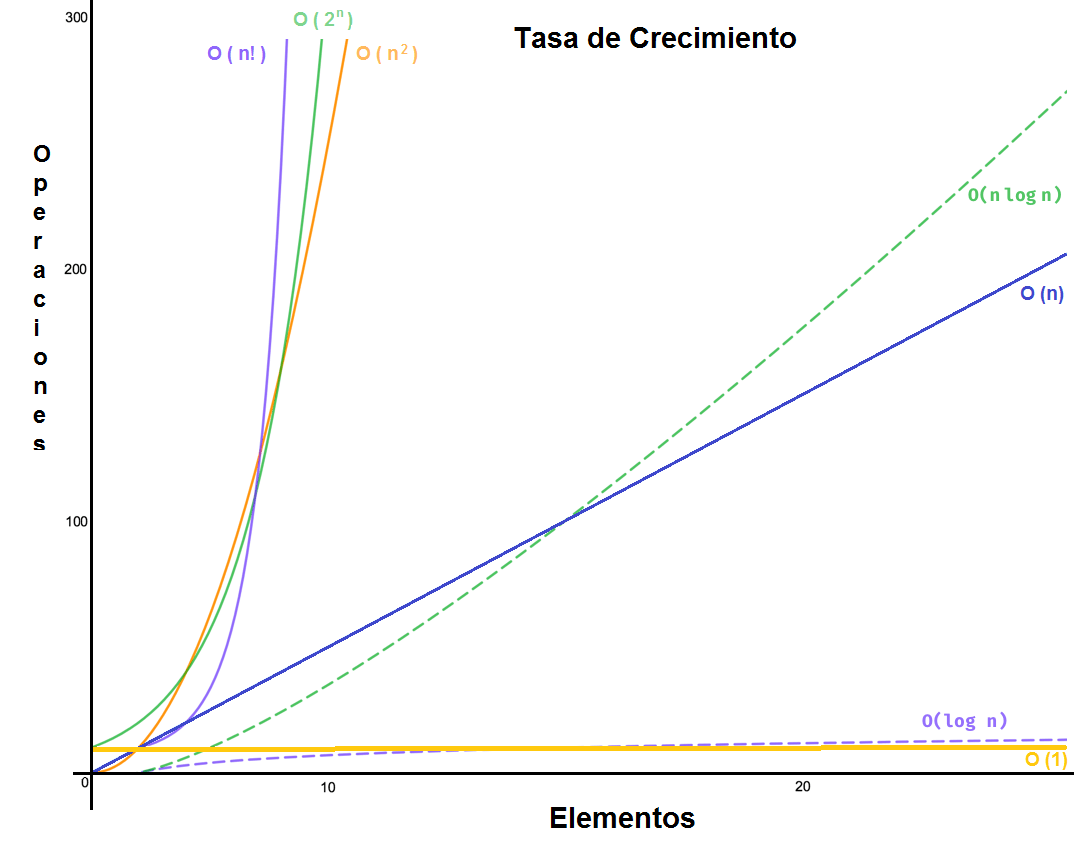
\includegraphics[scale = 0.4]{grafico-complejidad-computacionala3.png}
		\caption{Formas de crecimiento asint\'otico m\'as importantes}
		\label{fig:complejidad}
	\end{figure}
	
	\textbf{?`Comentar aqu\'i algo acerca de que hay que tener cuidado a la hora de comparar algoritmos en base a su coste asint\'otico? Por ejemplo con los algoritmos de Karatsuba, Toom-Cook y Sch\"onhage-Strassen para el producto.}
	\\
	
	Sin embargo, ?`qu\'e significa que un algoritmo sea eficiente? ?`Significa que toma un tiempo en $O(n\,log\,n)$? ?`$O(n^{2})$? Depender\'a del problema a resolver.
	\\
	
	Decimos que un algoritmo es eficiente (\textbf{citar Brassard}) si existe un polinomio $p(n)$ tal que el algoritmo puede resolver cualquier instancia del problema de tama\~{n}o \textit{n} en un tiempo $O(p(n))$. Se dice entonces que el algoritmo es de \textit{tiempo polin\'omico} y que los problemas que se resuelven con dicho algoritmo son resolubles en tiempo polin\'omico. Sin embargo, cuando el tiempo de ejecuci\'on de un algoritmo no se puede acotar mediante una f\'ormula polin\'omica, se dice que dicho algoritmo y su problema asociado son de \textit{tiempo exponencial}. Cuando solo se conocen algoritmos de tiempos exponenciales para resolver un problema, se dice que el problema es \textit{intratable}.
	\\
	
	Para lo que sigue, nos centraremos en el caso de los problemas de decisi\'on, que son aquellos problemas que tienen como respuesta s\'i o no, o equivalentemente, verdadero o falso.
	\\
	
	Todas estas consideraciones anteriores nos sirven de base para la introducci\'on de los siguientes conceptos:
	
	\begin{definicion}
		Una clase de complejidad es un conjunto de problemas que poseen la misma complejidad computacional (\textbf{citar wiki)}.
	\end{definicion}
	
	\begin{definicion}
		La clase de problemas de decisi\'on que pueden ser resueltos por una m\'aquina de Turing determinista en un tiempo polinomial es conocida como clase P (Poly\-nomial-time)
	\end{definicion}
	
	En t\'erminos generales, P corresponde a la clase de problemas que, de forma realista, se pueden \textbf{resolver} con un ordenador. Muchos de los problemas habituales (ordenaci\'on, b\'usqueda, etc.) pertenecen a esta clase.
	
	\begin{definicion}
		Llamamos clase NP (Non-Deterministic Polynomial-time) a aquella formada por los problemas de decisi\'on que son \textbf{verificables} por m\'aquinas de Turing no determinista en tiempos polin\'omicos.
	\end{definicion}
	
	Una relaci\'on evidente entre ambas clases es que $P \subset NP$, ya que si podemos resolver un problema en tiempo polin\'omico, evidentemente tambi\'en podemos verificarlo en tiempo polin\'omico.
	\\
	
	Otro importante subconjunto de la clase \textit{NP} son los problemas \textit{NP-completos}.(\textbf{citar wiki a continuaci\'on})
	
	\begin{definicion}
		Un problema de decisi\'on C es NP-completo si:
		\begin{enumerate}
			\item C $\in$ NP
			\item Todo problema de NP es \textbf{reducible polinomialmente} a C en tiempo polin\'omico.
		\end{enumerate}
	\end{definicion}
	
	Una reducci\'on polin\'omica de \textit{L} en \textit{C} es un algoritmo de tiempo polin\'omico que transforma instancias de \textit{L} en instancias de \textit{C}, de manera que la respuesta a \textit{C} es positiva si y solo si lo es la de \textit{L}. De forma general, la clase \textit{NP-completo} corresponde a la de los problemas que pueden verificarse de forma sencilla pero que, en el caso de que su espacio de soluciones sea muy grande, solo pueden resolverse por fuerza bruta. Algunos de los problemas que pertenecen a esta clase son el \textbf{problema de satisfacibilidad booleana} (SAT), el \textbf{problema de la mochila} (com\'unmente abreviado por KP), el \textbf{problema del ciclo hamiltoniano} o el \textbf{problema del viajante}. Esta clase tiene la propiedad (\textbf{citar wiki)} de que si alg\'un problema \textit{NP-completo} puede ser resuelto en tiempo polin\'omico, entonces todo problema en \textit{NP} tiene una soluci\'on en tiempo polin\'omico, es decir, $P = NP$.
	\\
	
	A pesar de a\~{n}os de investigaci\'on, la cuesti\'on de si $P = NP$ contin\'ua a\'un abierta y es considerado uno de los problemas del milenio. La importancia de este resultado radica en el hecho de que si $P \neq NP$, entonces los problemas \textit{NP-completos} son intratables, ya que si alg\'un problema en \textit{NP} requiere m\'as tiempo que uno polinomial, entonces uno \textit{NP-completo} tambi\'en.
	\\
	
	Una clase m\'as general de problemas no restringida a los problemas de decisi\'on es la clase de complejidad \textit{NP-dif\'icil} (\textit{NP-hard}). (\textbf{citar wiki para la def.})
	
	\begin{definicion}
		La clase de complejidad NP-dif\'icil es el conjunto que contiene a los problemas C tales que todo problema L en NP puede ser transformado polinomialmente en C.
	\end{definicion}
	
	Esta clase contiene a aquellos problemas que son, como m\'inimo, tan dif\'iciles como un problema de \textit{NP}. De esta forma, la clase de problemas \textit{NP-completo} puede definirse como la intersecci\'on entre las clases \textit{NP} y \textit{NP-dif\'icil}. (\textbf{imagen de wiki})
	
	\begin{figure}[h]
		\centering
		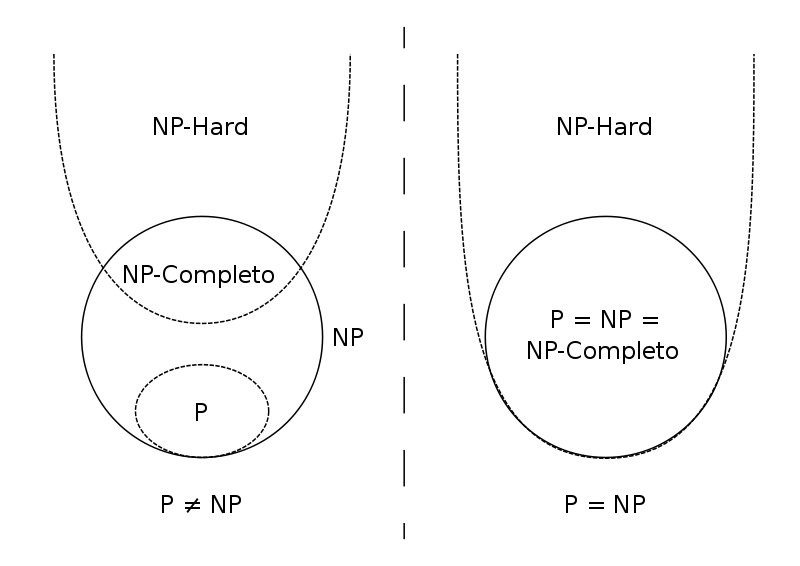
\includegraphics[scale = 0.4]{PNP.png}
		\caption{Diagrama de Euler de las clases de complejidad m\'as frecuentes}
		\label{fig:diagramaEuler}
	\end{figure}
	
	Un ejemplo de problema de optimizaci\'on combinatoria que es \textit{NP-dif\'icil} y que ser\'a el objeto central de estudio de este trabajo es el llamado \textit{problema de empaquetamiento} o \textbf{\textit{Bin Packing Problem}}.
	
	\section{Algoritmos heur\'{\i}sticos y metaheur\'{\i}sticos}
	
	Como ya se mencion\'o con anterioridad, para muchos problemas de optimizaci\'on combinatoria no se conocen algoritmos que sean capaces de obtener una soluci\'on \'optima en tiempo polinomial. Algunos incluso no admiten el uso de algoritmos de aproximaci\'on. En estos casos, nos vemos obligados a usar algoritmos heur\'{\i}sticos.
	\\
	
	Los m\'etodos heur\'{i}sticos son algoritmos que se limitan a proporcionar una "buena" soluci\'on del problema, no necesariamente \'optima, con un coste computacional razonable. Adem\'as, aunque un buen heur\'{\i}stico encuentre muy buenas soluciones para la mayor\'{\i}a de instancias de un problema, no hay garant\'{\i}a de que siempre encuentre una buena soluci\'on para todas las instancias del problema.
	\\
	
	Existen gran cantidad de m\'etodos heur\'{\i}sticos, lo cual hace que sea complicado dar una clasificaci\'on (\textbf{citar Rafael Mart\'{\i}}) de los mismos ya que, por ejemplo, muchos de ellos han sido dise\~{n}ados para resolver un problema concreto. No obstante, podemos dar una clasificaci\'on general donde ubicar a los algoritmos heur\'{\i}sticos m\'as conocidos:
	
	\begin{itemize}
		\item \textbf{M\'etodos de descomposici\'on.} El problema de partida se descompone en subproblemas m\'as sencillos de resolver, sin perder de vista que ambos pertenecen al mismo problema. (\textbf{Ejemplo?})
		\item \textbf{M\'etodos inductivos.} Estos m\'etodos parten de casos m\'as sencillos del problema general, de manera que analizan propiedades o t\'ecnicas que pueden generalizarse al problema completo. 
		\item \textbf{M\'etodos de reducci\'on.} Consiste en seleccionar propiedades que se verifican de forma general en las soluciones consideradas como buenas e introducirlas como restricciones del problema. La finalidad de estos m\'etodos es restringir el espacio de soluciones para simplificar el problema. El inconveniente que presentan estos m\'etodos, es la posibilidad de dejar fuera del espacio de soluciones nuevo aquellas soluciones \'optimas del problema original. 
		\item \textbf{M\'etodos constructivos.} Son m\'etodos que construyen paso a paso una soluci\'on del problema. Normalmente son m\'etodos deterministas y suelen estar basados en la mejor elecci\'on en cada iteraci\'on. (\textbf{Ejemplo?} - algoritmos voraces)
		\item \textbf{M\'etodos de b\'usqueda local.} A diferencia de los m\'etodos anteriores, los algoritmos de b\'usqueda o mejora local comienzan con una soluci\'on del problema y la mejoran progresivamente. El algoritmo realiza en cada iteraci\'on un movimiento de una soluci\'on a otra mejor. El m\'etodo finaliza cuando, para una soluci\'on, no existe ninguna otra accesible que la mejore. 
	\end{itemize}
	
	Cuando se resuelve un problema por m\'etodos heur\'isticos, como la optimalidad no est\'a garantizada, se debe medir la calidad de los resultados. Para ello existen diversos procedimientros, entre los cuales podr\'iamos destacar los siguientes:
	
	(\textbf{citar Orlando de Antonio Su\'arez})
	
	\begin{itemize}
		\item \textbf{Comparaci\'on con la soluci\'on \'optima.} Aunque normalmente se recurre al algoritmo aproximado por no existir un m\'etodo exacto para obtener el \'optimo, o por ser \'este computacionalmente muy costoso, en ocasiones puede que dispongamos de un m\'etodo que proporcione el \'optimo para un conjunto limitado de ejemplos. Este conjunto de ejemplos puede servir para medir la calidad del m\'etodo heur\'istico. Normalmente se mide, para cada uno de los ejemplos, la desviaci\'on porcentual de la soluci\'on heur\'istica frente a la \'optima, calculando posteriormente el promedio de dichas desviaciones.
		\item \textbf{Comparaci\'on con una cota.}  En ocasiones el \'optimo del problema no est\'a disponible ni siquiera para un conjunto limitado de ejemplos. Un m\'etodo alternativo de evaluaci\'on consiste en comparar el valor de la soluci\'on que proporciona el heur\'istico con una cota del problema (inferior si el problema es de minimizar y superior si es de maximizar). La bondad de esta medida depender\'a de la bondad de la cota, es decir, de c\'omo de cercana se encuentre del \'optimo del problema, por lo que de alguna manera, tendremos que tener informaci\'on de lo buena que es dicha cota. En caso contrario, la comparaci\'on propuesta no resulta de utilidad.
		\item \textbf{Comparaci\'on con un m\'etodo exacto truncado.} Para ello elegimos un m\'etodo exacto que resuelva el problema y establecemos un l\'imite de iteraciones o de tiempo m\'aximo conforme a una serie de criterios que nos garanticen que de esta forma obtenemos una buena soluci\'on. Una vez hecho esto, usamos esta soluci\'on para compararla con la que obtenemos seg\'un el heur\'istico. Evidentemente, en este caso suponemos que la resoluci\'on del problema mediante cualquier m\'etodo exacto es inabordable por el coste computacional que requiere.
		\item \textbf{Comparaci\'on con otros heur\'isticos.} Es un m\'etodo usado usalmente en problemas NP-duros para los que se conocen buenos heur\'isticos.
		\item \textbf{An\'alisis del peor caso.} Consiste en considerar los ejemplos que sean m\'as desfavorables para el algoritmo y acotar la m\'axima desviaci\'on respecto del \'optimo del problema. De esta forma, conseguimos acotar el resultado del algoritmo para cualquier ejemplo. Lo malo es que los resultados no suelen ser representativos del comportamiento medio del algoritmo.
	\end{itemize}
	
	Si bien todos estos m\'etodos han contribuido a ampliar nuestro conocimiento para la resoluci\'on de problemas reales, los m\'etodos constructivos y los de b\'usqueda local constituyen la base de los procedimientos metaheur\'isticos.
	\\
	
	Los metahur\'isticos son m\'etodos para dise\~{n}ar y/o mejorar los heur\'isticos en los que estos m\'etodos cl\'asicos no son efectivos a la hora de resolver un problema dif\'icil de optimizaci\'on combinatoria. Son algoritmos h\'ibridos que combinan conceptos de distintos campos como la gen\'etica, la biolog\'ia, la f\'isica, las matem\'aticas, la inteligencia artificial o la neurolog\'ia, por ejemplo. Algunos de los m\'as comunes son los siguientes:
	
	\begin{itemize}
		\item \textbf{Metaheur\'isticos inspiradas en la f\'isica:} Como ya se ha mencionado con anterioridad, el recocido simulado  es un ejemplo de este tipo de algoritmos. Es una t\'ecnica de b\'usqueda inspirada en el proceso de calentamiento y posterior enfriamiento de un metal para obtener estados de baja energ\'ia en un s\'olido. 
		\item \textbf{Metaheur\'isticos inspiradas en la evoluci\'on:} Son m\'etodos que van construyendo una soluci\'on en cada iteraci\'on. Consiste en generar, seleccionar, combinar y reemplazar un conjunto de soluciones en la b\'usqueda de la mejor soluci\'on. Un ejemplo de estos m\'etodos son los algoritmos gen\'eticos. 
		\item \textbf{Metaheur\'isticos inspiradas en la biolog\'ia:} Un ejemplo relativamente reciente de este tipo de algoritmos es la optimizaci\'on basada en colonias de hormigas (ant colony optimization). Se inspira en el comportamiento estructurado que siguen las colonias de hormigas donde los individuos se comunican entre s\'i por medio de las feromonas; la repetici\'on de recorridos por los individuos establece el camino m\'as adecuado entre su nido y su fuente de alimentos. El m\'etodo consiste en simular la comunicaci\'on indirecta que utilizan las hormigas para establecer el camino m\'as corto, guardando la informaci\'on aprendida en una matriz de feromonas.
	\end{itemize}
	
	
	
	
	\chapter{Problema del empaquetamiento (Bin Packing)}
	
	\section{Introducci\'on}
	Existen diversas formulaciones para el problema de Bin Packing, al que nos referiremos de ahora en adelante de manera abreviada como BP o BPP. De forma sencilla, podemos enunciarlo como:
	
	\begin{center}
		Dados \textit{n} objetos de tama\~{n}o $w_{1},..., w_{n}$, queremos encontrar el menor n\'umero de cubos de capacidad \textit{c} necesario para empaquetar todos los objetos.
	\end{center}
	
	A los objetos $w_{i}$ anteriores se les denomina habitualmente pesos. Son m\'ultiples las aplicaciones que tienen los problemas de tipo BP, adem\'as que podemos considerar variantes multidimensionales: desde el llenado de contenedores y/o camiones con restricciones de volumen y peso a la creaci\'on de copias de seguridad de archivos o una asignaci\'on eficiente de la memoria de un ordenador. 
	\\
	
	Como vemos, es un problema d\'ificil de resolver debido a que su complejidad crece exponencialmente con el n\'umero de objetos a almacenar y variables a considerar, como por ejemplo si dichos objetos fueran tridimensionales y tuvi\'eramos que considerar su volumen y su peso a la hora de imponer las restricciones del problema. Resulta aqu\'i visible la dificultad que presentan los problemas de optimizaci\'on combinatoria y la necesidad de desarrollar algoritmos suficientemente buenos que puedan resolverlos en tiempos aceptables.
	
	\begin{observacion}
		Cuando el n\'umero de cubos se limita a uno y cada objeto se caracteriza por su peso, el problema de maximizar el peso de los objetos que pueden caber en el contenedor se conoce como el  ya mencionado problema de la mochila.
	\end{observacion}
	
	El BPP tambi\'en puede considerarse como un caso especial del \textit{cutting stock problem}, cuyo origen est\'a asociado a la industria maderera: (citar wiki)
	\\
	
	Consideremos una lista de \textit{m} \'ordenes para las cuales se requiere $q_{j}$, $j = 1,...,m$ piezas para cada una. Posteriormente, se construye una lista de todas las combinaciones posibles de los recortes (frecuentemente llamados \textit{patrones}), asociando a cada uno de ellos una variable entera positiva $x_{i}$ que representa cuantas veces ser\'a utilizado cada patr\'on. Entonces, el problema de programaci\'on lineal entera se modeliza matem\'aticamente como
	\newpage
	
	$$ min \sum_{i=1}^{n}c_{i}x_{i} $$
	$$ s.a\, \sum_{i=1}^{n}a_{ij}x_{i},\, \forall j=1,...,m $$
	$$ x_{i}\in \mathbb{Z^{+}},\, \forall i=1,...,n $$
	\\
	donde $a_{ij}$ es el n\'umero de veces que en la orden \textit{j} aparece el patr\'on \textit{i} y $c_{i}$ es el costo (a menudo llamado \textit{residuo}) del patr\'on \textit{i}.
	\\
	
	As\'i, procedemos a continuaci\'on a formular matem\'aticamente el problema BP.
	\\
	
	Sean \textit{n} objetos (items) y \textit{n} cubos (bins), donde
	
	$$w_{j} = \mbox{peso del item \textit{j}},$$
	$$c = \mbox{capacidad de cada cubo},$$
	\\
	entonces 
	
	$$ min \sum_{i=1}^{n}y_{i} $$
	$$ s.a\, \sum_{j=1}^{n}w_{j}x_{ij} \leq cy_{i},\, \forall i=1,...,n $$
	$$ \sum_{i=1}^{n}x_{ij} = 1,\, \forall j=1,...,n $$
	\\
	donde
	
	\[y_{i} = \left\{\begin{array}{ll}
		1 \hspace{0.5cm} \text{si se usa el bin \textit{i}}\\
		0 \hspace{0.5cm} \text{en otro caso}
	\end{array}\right.\]
	\\
	\[x_{ij} = \left\{\begin{array}{ll}
		1 \hspace{0.5cm} \text{si el item \textit{j} se asigna al bin \textit{i}}\\
		0 \hspace{0.5cm} \text{en otro caso}
	\end{array}\right.\]
	\\
	Supondremos, adem\'as, que los pesos $w_{j}$ son enteros positivos. Por lo tanto, sin p\'erdida de generalidad, podemos suponer que
	
	$$ c \mbox{ es un entero positivo,} $$
	$$ w_{j} \leq c,\, \forall j = 1,...,n. $$
	\\
	Si alg\'un item no verifica la \'ultima suposici\'on, entonces el problema es trivialmente imposible.
	\\
	
	En lo que sige, propondremos una serie de algoritmos con los que aproximar las soluciones de distintas instancias del problema BP, a la par que analizaremos c\'omo de buenos son y qu\'e coste computacional tienen. Para ello, el primer tipo de m\'etodos que analizaremos ser\'an los algoritmos voraces (\textit{greedy alghorithm}).
	
	\section{Algoritmos voraces}
	Por algoritmos voraces se entienden aquellos algoritmos que siguen un esquema de resoluci\'on llamado m\'etodo voraz. Dicho esquema consiste esencialmente en construir una soluci\'on de forma incremental, tomando decisiones localmente \'optimas en cada paso, lo cual no implica que la soluci\'on final sea globalmente \'optima. Esquema que siguen algoritmos como, por ejemplo, el m\'etodo del gradiente, los algoritmos gen\'eticos o los algoritmos de cristalizaci\'on simulada. Los algoritmos que siguen este m\'etodo son, en general, los que menos dificultades plantean a la hora de implementar y comprobar su funcionamiento, y suelen aplicarse en problemas de optimizaci\'on.
	\\
	
	Frecuentemente, los algoritmos de tipo greedy y los problemas que pueden resolver, se caracterizan por la mayor\'ia de las siguientes caracter\'isticas (\textbf{citar Brassard}):
	
	\begin{itemize}
		\item Tenemos que resolver un problema de optimizaci\'on y, para construir su soluci\'on, tenemos un conjunto de candidatos: en el caso que nos ata\~{n}e, esos candidatos resultan ser los objetos que queremos introducir en los cubos.
		\item A medida que el algoritmo avanza, tenemos otros dos conjuntos. Por un lado, tenemos el conjunto formado por los candidatos que ya han sido considerados y elegidos, mientras que por otro tenemos el conjunto con los candidatos que han sido considerados y rechazados.
		\item Hay una funci\'on que verifica si un conjunto particular de candidatos es una soluci\'on del problema, independientemente de si dicha soluci\'on es la \'optima.
		\item Hay otra funci\'on que verifica si un conjunto de candidatos es factible, es decir, si es posible o no completar el conjunto a\~{n}adiendo m\'as candidatos hasta obtener al menos una soluci\'on del problema. De nuevo, esta funci\'on tampoco tiene en cuenta la optimalidad de dicha soluci\'on.
		\item Una funci\'on m\'as, llamada funci\'on de selecci\'on, que indica en cada momento cual de los candidatos restantes, que no han sido elegidos ni rechazados, es el que podr\'ia ser el mejor.
		\item Finalmente, una funci\'on objetivo que nos proporciona el valor de la soluci\'on que hemos encontrado. En nuestro problema de BP, dicha funci\'on
		es el n\'umero de bins a minimizar y, a diferencia de las tres funciones
		anteriores, la funci\'on objetivo no aparece expl\'icitamente en el algoritmo.
	\end{itemize}
	
	Un algoritmo voraz avanza paso a paso. Esto quiere decir que, inicialmente,
	el conjunto de los candidatos elegidos est\'a vac\'io. Luego, en cada paso, la funci\'on de selecci\'on elige al mejor candidato restante sin parar a considerar si lo introducimos o no en el conjunto anterior. Si el conjunto ampliado de candidatos elegidos ya no es factible, rechazamos el candidato que estamos considerando actualmente. En este caso, el candidato con el que hemos probado y que ha sido rechazado no se vuelve a considerar de nuevo. En cambio, si el conjunto ampliado es factible, a\~{n}adimos el candidato al conjunto de los candidatos elegidos. Cada vez que ampliamos dicho conjunto, verificamos si en ese momento este conjunto es una soluci\'on del problema. De esta forma, un algoritmo voraz se ver\'ia de la siguiente forma:
	\\
	
	\noindent\fbox{
		\begin{minipage}{0.5\textwidth}
			\begin{algorithmic}
				
				\State{funci\'on greedy (C: set): set}
				\State{//C es el conjunto de los candidatos}
				\State{//Construimos la soluci\'on en el conjunto S}
				\State{S = $\emptyset$}\
				\While{(C $\neq \emptyset$ \textbf{y no} solucion(S))}
				\State{$x \longleftarrow seleccionar(C)$}
				\State{$C \longleftarrow C-\{x\}$}
				\If{($factible(S\cup \{x\})$)}
				\State{$S \longleftarrow S\cup \{x\}$}
				\EndIf
				\EndWhile
				\If{(solucion(S))}
				\State{\textbf{return} S}
				\Else
				\State{\textbf{return} "No hay soluci\'on"}
				\EndIf
				
			\end{algorithmic}
		\end{minipage}
	}
	\\\\
	
	A continuaci\'on, pasamos a presentar los algoritmos voraces con los que ofreceremos distintas soluciones del problema del BP. Daremos una breve explicaci\'on del funcionamiento de los algoritmos, sus pseudoc\'odigos y analizaremos sus complejidades. 
	
	
	\subsection{Primeras aproximaciones}
	\subsubsection{Next Fit}
	Este algoritmo es el m\'as sencillo de implementar y con el que podemos obtener una r\'apida soluci\'on del problema, aunque no muy buena. Funciona de la siguiente manera: comenzamos con una soluci\'on en la que no tenemos ning\'un cubo. A continuaci\'on, seleccionamos el primer objeto de la lista de objetos que queremos introducir en los cubos y lo introducimos en un nuevo cubo dado que es el primer elemento seleccionado. Para los siguientes objetos, el algoritmo comprueba si podemos introducir el elemento seleccionado en el \'ultimo cubo creado. Si se puede, lo introducimos. En otro caso, creamos un cubo nuevo y lo introducimos.
	\\
	
	Vemos que, aunque es un algoritmo que nos permite obtener una soluci\'on de manera sencilla y r\'apida (puesto que no hay muchas comprobaciones que realizar), no resulta muy eficiente como veremos. As\'i, el pseudoc\'odigo del algoritmo ser\'ia el siguiente:
	
	\noindent\fbox{
		\begin{minipage}{\textwidth}
			\begin{algorithmic}
				
				\State{nextFit (capacity: Int, items: Array[Int]): Array[Bin]}
				\State{//capacity es la capacidad de los cubos}
				\State{//items es un array que almacena los elementos que introduciremos en los cubos}
				\State{//El array solution almacenar\'a los cubos y current ser\'a el \'ultimo cubo creado}
				\State{solution = $\emptyset$}\
				\State{current = new Bin(capacity)}\
				\For{(item $\leftarrow$ items)}
				\If{(item cabe en current)}
				\State{A\~{n}adimos el item a current}
				\Else
				\State{A\~{n}adimos current a solution}
				\State{current = new Bin(capacity)}
				\State{A\~{n}adimos el item a current}
				\EndIf
				\EndFor
				\State{A\~{n}adimos el \'ultimo cubo creado a solution}
				\State{\textbf{return} solution}
				
			\end{algorithmic}
		\end{minipage}
	}
	\\\\
	
	Observemos que, dada una lista de \textit{n} pesos, el algoritmo hace una \'unica comprobaci\'on por cada iteraci\'on. Por lo tanto, tenemos que la complejidad del algoritmo es \textit{O(n)}, con lo que el tiempo necesario para la resoluci\'on del problema se incrementa de forma lineal conforme lo hace el n\'umero de elementos que tenemos que introducir en los cubos. As\'i pues, como primera aproximaci\'on, ser\'ia un algoritmo \'util, r\'apido y f\'acil de resolver para instancias peque\~{n}as del problema en las que no estamos interesados en obtener el \'optimo. Adem\'as, su sencillez nos permite conseguir resultados como el siguiente:
	
	\begin{teorema}
		Sea M el n\'umero de cubos de capacidad c necesarios para empaquetar una lista de n objetos de forma \'optima. Entonces el algoritmo Next Fit usar\'a a lo sumo 2M cubos.
	\end{teorema}
	
	\begin{proof}
		\hfill \break
		
		Haremos la demostraci\'on para el caso par. Sea \textit{k} el n\'umero de cubos de la soluci\'on obtenida al aplicar el algoritmo Next Fit y sea $B_{i}$ el cubo i-\'esimo de la soluci\'on. Denotemos por $s(B_{i})$ a la suma de los pesos de los objetos empaquetados en el cubo $B_{i}$.
		\\
		
		Entonces, para cualesquiera dos cubos adyascentes $B_{i}$ y $B_{i+1}$ se verifica que
		$$s(B_{i}) + s(B_{i+1}) > c$$
		
		Por lo tanto, tenemos que
		$$s(B_{1}) + s(B_{2}) > c,\, s(B_{3}) + s(B_{4}) > c,\, ...,\, s(B_{k-1}) + s(B_{k}) > c.$$
		
		Con lo que, si sumamos todas estas desigualdades llegamos a
		$$\sum_{i=1}^{k}s(B_{i}) > \frac{k}{2}c.$$
		
		Adem\'as, como cualquier cubo de la soluci\'on verifica 
		$$s(B_{i}) \leq c,$$
		
		llegamos a 
		$$kc \geq \sum_{i=1}^{k}s(B_{i}) > \frac{k}{2}c.$$
		
		Por otro lado, observemos que para la soluci\'on \'optima del problema tambi\'en se verifica las desigualdades anteriores, es decir,
		$$Mc \geq \sum_{i=1}^{M}s(B_{i}).$$
		
		Por \'ultimo, teniendo en cuenta que
		$$\sum_{i=1}^{M}s(B_{i}) = \sum_{i=1}^{k}s(B_{i}),$$
		
		llegamos a 
		$$Mc \geq \sum_{i=1}^{M}s(B_{i}) = \sum_{i=1}^{k}s(B_{i}) > \frac{k}{2}c,$$
		
		de donde deducimos que
		$$Mc > \frac{k}{2}c \Longrightarrow 2M > k$$
		
		Podemos ver una prueba m\'as general en \cite{Graduatecourse}.
		
	\end{proof}
	
	
	\subsubsection{First Fit}
	Podr\'iamos considerar a este algoritmo como un primer intento de mejorar el m\'etodo anterior ya que, aunque no reconsideremos las decisiones tomadas (es decir, si alguno de los items introducidos en los cubos existentes deber\'ia introducirse en otro cubo), que es la idea b\'asica de los algortimos voraces, s\'i que vamos llenando "mejor" los cubos que se van creando en las iteraciones del algoritmo. Adem\'as, posteriormente \'este ser\'a uno de los algortimos que usaremos como base para implemententar mejores t\'ecnicas de resoluci\'on del problema del BP.
	\\
	
	El algoritmo es el siguiente: empezamos igual que en el caso anterior; partimos de una soluci\'on que no tiene ningu\'un cubo. Seleccionamos el primer elemento de nuestra lista de objetos a introducir en los cubos y creamos un primer cubo donde a\~{n}adimos el elemento. Para los siguientes elementos, recorremos nuestra soluci\'on de cubos y a\~{n}adimos el elemento en el primer cubo que encontremos donde quepa el objeto. Si no hay ning\'un cubo en el que quepa el elemento seleccionado, creamos un nuevo cubo y lo introducimos.
	\\
	
	De esta forma, el pseudoc\'odigo del algoritmo ser\'ia el siguiente:
	\\
	
	\noindent\fbox{
		\begin{minipage}{\textwidth}
			\begin{algorithmic}
				
				\State{firstFit (capacity: Int, items: Array[Int]): Array[Bin]}
				\State{//capacity es la capacidad de los cubos}
				\State{//items es un array que almacena los elementos que introduciremos en los cubos}
				\State{//El array solution almacenar\'a los cubos y current ser\'a el \'ultimo cubo creado}
				\State{//Inicializamos el algoritmo con el array de soluciones teniendo un cubo vac\'io}
				\State{current = new Bin(capacity)}\
				\State{A\~{n}adimos el cubo vac\'io a solution}\
				\For{(item $\leftarrow$ items)}
				\State{i = 0}
				\While{(item \textbf{no} est\'e a\~{n}adido \textbf{y} i $\leq$ tama\~{n}o de solution)}
				\If{(El item cabe en el cubo i-\'esimo)}
				\State{A\~{n}adimos el item en el cubo i-\'esimo}
				\Else
				\State{i = i + 1}
				\EndIf
				\EndWhile
				\If{(El item no se ha a\~{n}adido a ning\'un cubo)}
				\State{current = new Bin(capacity)}
				\State{A\~{n}adimos el item a current}
				\State{A\~{n}adimos el cubo current a solution}
				\EndIf
				\EndFor
				\State{\textbf{return} solution}
				
			\end{algorithmic}
		\end{minipage}
	}
	\\\\
	
	Como mencionamos anteriormente, este algoritmo conseguimos mejorar la soluci\'on obtenida seg\'un el m\'etodo Next Fit, pero esto implica que la complejidad algor\'itmica se incrementa. Dada una lista de \textit{n} elementos, el bucle for itera sobre cada uno de ellos, por lo que la complejidad introducida a priori por el bucle es \textit{O(n)}. Pero, a su vez, en cada iteraci\'on el bucle while recorre en el peor de los casos toda la lista de cubos, con lo que su complejidad es tambi\'en \textit{O(n)}. Por lo tanto, la complejidad del algoritmo resulta ser $O(n^{2})$.
	\\
	
	\begin{teorema}
		Sea M el n\'umero de cubos de capacidad c necesarios para empaquetar una lista de n objetos de forma \'optima. Entonces el algoritmo First Fit no usa m\'as de 1,7M cubos.
	\end{teorema}
	
	\begin{proof}
		\hfill \break
		Se omite la demostraci\'on de este resultado debido a su larga extensi\'on y a que requiere de unos cuantos resultados previos que se alejan del prop\'osito de lo que aqu\'i tratamos. No obstante, podemos encontrarla en \cite{1.7OPT}
	\end{proof}
	
	
	\subsubsection{Best Fit}
	Este es el primero de los algoritmos que intenta ofrecernos una mejora "considerable" a la hora de llenar los cubos ya que no solo intenta ir llenando todos los cubos en cada iteraci\'on, sino que los llena de la mejor forma posible, entendiendo esa forma mejor como aquella en la que el elemento seleccionado rellena mejor en el cubo. Al igual que para First Fit y los m\'etodos posteriores, las mejoras que conseguimos en busca de la soluci\'on \'optima o una aproximada, aparecen a costa de incrementar la complejidad del algoritmo.
	\\
	
	De esta forma, el algoritmo Best Bit es: seleccionamos el primer objeto de nuestra lista, creamos un nuevo cubo con la capacidad dada en el problema e introducimos el objeto. Para los siguientes elementos buscamos el cubo cuya capacidad restante sea menor y en el que, adem\'as, quepa el elemento. Si encontramos un cubo que cumpla esta condici\'on introducimos el objeto. En otro caso, creamos un cubo nuevo y lo introducimos.
	\\
	
	Obs\'ervese que el cubo que verifique las condiciones dadas para introducir un nuevo elemento no tiene por qu\'e ser \'unico. Por lo tanto, a la hora de implementar el algoritmo iremos insertando los cubos en nuestra soluci\'on de manera ordenada, con lo que cuando vayamos a seleccionar en qu\'e cubo introducimos un nuevo elemento cuando haya m\'as de una elecci\'on posible, lo haremos eligiendo el primer cubo que encontremos. As\'i, el pseudoc\'odigo del algoritmo queda como sigue: 
	\\
	
	\noindent\fbox{
		\begin{minipage}{\textwidth}
			\begin{algorithmic}
				
				\State{bestFit (capacity: Int, items: Array[Int]): Array[Bin]}
				\State{//capacity es la capacidad de los cubos}
				\State{//items es un array que almacena los elementos que introduciremos en los cubos}
				\State{//El array solution almacenar\'a los cubos y current ser\'a el \'ultimo cubo creado}
				\State{//Inicializamos el algoritmo con el array de soluciones sin ning\'un cubo}
				\State{//targetBin es la posici\'on en solution del cubo con la menor capacidad restante que es mayor o igual que el peso del item seleccionado}
				\State{//smallerThanTarget es un m\'etodo de b\'usqueda binaria con el que, dado un array de cubos ordenados seg\'un sus capacidades restantes de forma creciente y un elemento, encuentra la posici\'on del menor elemento del array que es mayor o igual que el elemento dado}
				\State{solution = $\emptyset$}\
				\For{(item $\leftarrow$ items)}
				\State{targetBin = 1 + smallerThanTarget(item, solution)}
				\If{(targetBin $\geq$ 0 \textbf{y} targetBin $\leq$ longitud de solution - 1)}
				\State{A\~{n}adimos el item en el cubo que se encuentra en la posicion targetBin}
				\State{Reordenamos el array solution de menor a mayor capacidad restante}
				\Else
				\State{current = new Bin(capacity)}
				\State{A\~{n}adimos el item en el cubo current}
				\State{A\~{n}adimos el cubo current en solution}
				\State{Reordenamos el array solution de menor a mayor capacidad restante}
				\EndIf
				\EndFor
				\State{\textbf{return} solution}
				
			\end{algorithmic}
		\end{minipage}
	}
	\\\\
	
	Como ya veremos en el cap\'itulo dedicado a explicar la implementaci\'on de los m\'etodos aqu\'i descritos, lo primero que debemos tener en cuenta para analizar la complejidad de este algoritmo es que, en cada iteraci\'on, para localizar el cubo donde el objeto seleccionado quede m\'as ajustado realizamos una b\'usqueda binaria con el m\'etodo \textit{smallerThanTarget}, que es \textit{O(log n)}. Por otro lado, tras insertar el elemento, la capacidad del cubo disminuir\'a, con lo que tendremos que desplazarlo a la izquierda (ya que en nuestra implementaci\'on ordenaremos los cubos de menor a mayor capacidad restante) para seguir manteniendo los cubos en orden. En el peor de los casos, este desplazamiento ser\'a \textit{O(n)} si, por ejemplo, tenemos que desplazar un cubo que est\'a en el extremo derecho al extremo izquierdo.
	\\
	
	Por lo tanto, cada iteraci\'on en la que insertamos un nuevo elemento ser\'a \textit{O(log n)} + \textit{O(n)} = \textit{O(n)}. De esta forma, como tenemos que insertar \textit{n} elementos, el coste total del algoritmo ser\'a $n \cdot O(n) = O(n^{2})$.
	
	\subsubsection{Worst Fit}
	El m\'etodo Worst Fit es una variante del algoritmo Best Fit. Mientras que en el m\'etodo Best Fit vamos introduciendo los pesos en aquellos cubos que quepan y que tengan la menor capacidad restante posible, en el Worst Fit los introducimos en los cubos que quepan y que, adem\'as, tengan la mayor capacidad restante de entre todos ellos. Tambi\'en, al igual que en el m\'etodo Best Fit, a la hora de implementar el algoritmo tenemos la soluci\'on con los cubos ordenados de menor a mayor capacidad restante. As\'i, como tenemos que elegir aquel cubo con la mayor capacidad restante, lo \'unico que tendremos que comprobar en cada iteraci\'on del algoritmo es que el peso seleccionado quepa en el \'ultimo cubo de la soluci\'on.
	\\
	
	As\'i, el algoritmo quedar\'ia: inicializamos el algoritmo igual que en Best Fit, partiendo de una soluci\'on que tiene un cubo en el cual introducimos el primer peso. A continuaci\'on, para cada elemento buscamos aquel cubo con la mayor capacidad restante y en el que quepa el elemento. Si lo encontramos, introducimos el peso. En otro caso creamos un cubo nuevo, introducimos el elemento y a\~{n}adimos el cubo a la soluci\'on. Por lo tanto, el pseudoc\'odigo del algoritmo quedar\'ia como:
	\\
	
	\noindent\fbox{
		\begin{minipage}{\textwidth}
			\begin{algorithmic}
				
				\State{worstFit (capacity: Int, items: Array[Int]): Array[Bin]}
				\State{//capacity es la capacidad de los cubos}
				\State{//items es un array que almacena los elementos que introduciremos en los cubos}
				\State{//El array solution almacenar\'a los cubos y current ser\'a el \'ultimo cubo creado}    
				\State{//targetBin es la posici\'on en solution del cubo con la menor capacidad restante que es mayor o igual que el peso del item seleccionado}
				\State{//Inicializamos el algoritmo con el array de soluciones sin ning\'un cubo}
				\State{solution = $\emptyset$}\
				\For{(item $\leftarrow$ items)}
				\If{(solution no est\'a vac\'io \textbf{y} el item cabe en el \'ultimo cubo de solution)}
				\State{A\~{n}adimos el item en el cubo que se encuentra en la \'ultima posici\'on}
				\State{Reordenamos el array solution de menor a mayor capacidad restante}
				\Else
				\State{current = new Bin(capacity)}
				\State{A\~{n}adimos el item en el cubo current}
				\State{A\~{n}adimos el cubo current en solution}
				\State{Reordenamos el array solution de menor a mayor capacidad restante}
				\EndIf
				\EndFor
				\State{\textbf{return} solution}
				
			\end{algorithmic}
		\end{minipage}
	}
	\\\\
	
	El razonamiento que tenemos que seguir para analizar la complejidad de este algoritmo es pr\'acticamente an\'alogo al caso del algoritmo Best Fit. A diferencia del algoritmo anterior, en este m\'etodo no tenemos que realizar una b\'usqueda binaria para localizar el cubo donde insertar el objeto, sino que siempre lo intentamos insertar en el \'ultimo cubo de nuestra soluci\'on, lo cual pareciera que reduce la complejidad del algoritmo. Sin embargo, una vez insertado el elemento en el cubo, ya sea en el \'ultimo cubo de la soluci\'on o creando uno nuevo, de nuevo la capacidad de dicho cubo disminuir\'a y tendremos que desplazarlo a la izquierda si as\'i fuera necesario. En el peor de los casos, este desplazamiento ser\'a $O(n)$ si tenemos un cubo por elemento y tuvi\'eramos que desplazar el cubo (siempre desde el extremo derecho) al extremo izquierdo.
	\\
	
	Esto significa que cada iteraci\'on en la que insertamos un elemento, su complejidad ser\'a $O(n)$ y, dado que tenemos que insertar \textit{n} n elementos, el coste total del algoritmo ser\'a $n \cdot O(n) = O(n^{2})$.
	\\
	
	De aqu\'i en adelante los m\'etodos que emplearemos para buscar mejores soluciones para el problema del BP utilizar\'an de base las t\'ecnicas anteriores. No obstante, antes de llegar a ellos podemos mencionar una serie de variaciones de los algoritmos anteriores que, en funci\'on de la instancia del problema que estemos considerando, pueden ofrecer mejores soluciones que los algoritmos que hemos visto hasta ahora.
	\\
	
	\subsection{Algunas variaciones de los m\'etodos anteriores}
	\subsubsection{Next k Fit}
	
	El m\'etodo Next k Fit podr\'ia considerarse como una generalizaci\'on del m\'etodo Next Fit. La diferencia es que mientras que en el m\'etodo Next Fit solo tenemos "abierto" el \'ultimo cubo de la soluci\'on (es decir, solo miramos el \'ultimo a la hora de comprobar si podemos introducir un nuevo elemento o si creamos un cubo nuevo donde introducirlo), en este m\'etodo tenemos abierto los \textit{k} \'ultimos cubos. As\'i, dada una soluci\'on de cubos de longitud \textit{n} y un nuevo elemento a introducir en ellos, comenzar\'iamos comprobando si el elemento cabe en el cubo de posici\'on $n-(k-1)$; si cabe lo introducimos, en otro caso pasamos al cubo de posici\'on $n-(k-2)$ y as\'i sucesivamente hasta llegar al \'ultimo cubo. Como dijimos con anterioridad, el m\'etodo Next Fit no es m\'as que un caso particular de este m\'etodo cuando $k=1$.
	\\
	
	Podemos apreciar a simple vista que m\'etodos de este tipo podr\'ian mejorar al algoritmo Next Fit cuando $k>1$ dado que nos permite "llenar" mejor los cubos de la soluci\'on al comprobar si un elemento dado cabe en m\'as de un cubo.
	\\
	
	\noindent\fbox{
		\begin{minipage}{\textwidth}
			\begin{algorithmic}
				
				\State{nextKFit (k: Int, capacity: Int, items: Array[Int]): Array[Bin]}
				\State{//capacity es la capacidad de los cubos}
				\State{//items es un array que almacena los elementos que introduciremos en los cubos}
				\State{//El array solution almacenar\'a los cubos y current ser\'a el \'ultimo cubo creado}    
				\State{//k es un n\'umero entero que representa el n\'umero de cubos que permanecer\'an abiertos en cada iteraci\'on}
				\State{//Inicializamos el algoritmo con el array de soluciones sin ning\'un cubo}
				\State{solution = $\emptyset$}\
				\State{current = new Bin(capacity)}\
				\For{(item $\leftarrow$ items)}
				\If{(solution = $\emptyset$)}
				\If{(puedo a\~{n}adir el item en el cubo current)}
				\State{A\~{n}adimos el item en el cubo current}
				\Else
				\State{A\~{n}adimos el cubo current en solution}
				\State{current = new Bin(capacity)}
				\State{A\~{n}adimos el item en el cubo current}
				\State{A\~{n}adimos el cubo current en solution}
				\EndIf
				\ElsIf{(solution $\neq \emptyset$ \textbf{y} solution.length $<$ k)}
				\State{aux = 0}
				\While{(aux $\leq k-1$  \textbf{y} el item \textbf{no} est\'e a\~{n}adido)}
				\If{(el item cabe en el cubo que se encuentra en la posici\'on aux)}
				\State{A\~{n}ado el elemento al cubo}
				\Else
				\State{aux += 1}
				\EndIf
				\EndWhile
				\If{(el item no se ha a\~{n}adido en ning\'un cubo)}
				\State{current = new Bin(capacity)}\
				\State{A\~{n}adimos el item en el cubo current}
				\State{A\~{n}adimos el cubo current en solution}
				\EndIf
				\Else
				\State{i = 1}
				\While{(el item no est\'e a\~{n}adido y no hayamos comprobado los \'ultimos k cubos)}
				\If{(podemos a\~{n}adir el item en el cubo (k-i)-\'esimo)}
				\State{Introducimos el item en el cubo (k-i)-\'esimo}
				\Else
				\State{i += 1}
				\EndIf
				\EndWhile
				\If{(el item no se ha a\~{n}adido)}
				\State{current = new Bin(capacity)}
				\State{A\~{n}adimos el item en el cubo current}
				\State{A\~{n}adimos el cubo current en solution}
				\EndIf
				\EndIf
				\EndFor
				\State{\textbf{return} solution}
				
			\end{algorithmic}
		\end{minipage}
	}
	\\\\
	
	La complejidad de este algoritmo es id\'entica al Next Fit. Esto se debe a que el bucle for recorre toda la lista de objetos, luego al igual que en los algoritmos previos, su complejidad es \textit{O(n)}. Por otra parte, el bucle while itera, a lo sumo, k veces, con lo que la complejidad del algoritmo es $k\cdot O(n) = O(n)$ ya que k es una constante.
	
	\subsubsection{Algoritmos de tipo decreasing/increasing}
	Este tipo de algoritmos recoge los m\'etodos ya planteados y les realiza una peque\~{n}a variaci\'on que es, b\'asicamente, ordenar antes de empezar el proceso la lista de objetos a introducir en los cubos de manera descendente seg\'un sus pesos. As\'i, este tipo de variaci\'on da lugar a los algoritmos \textit{First Fit Decreasing}, \textit{Best Fit Decreasing} o incluso \textit{Worst Fit Decreasing}. 
	\\
	
	L\'ogicamente, el resto de m\'etodos voraces que presentamos en este trabajo tambi\'en son susceptibles de introducir este cambio en su algoritmo, pero su uso no suele ser tan com\'un ni tampoco introducen mejoras considerables en la obtenci\'on de mejores resultados. Por otro lado, en lugar de ordenar la lista de objetos de manera descendente, tambi\'en podr\'ia hacerse de forma ascendente, lo cual podr\'ia llegar a resultar beneficioso seg\'un la instancia del problema que se estuviera tratando de resolver.
	\\
	
	En cuanto a la complejidad del algoritmo resultante cuando aplicamos este cambio, podemos observar que no var\'ia en absoluto para los m\'etodos que estamos considerando. Esto es as\'i porque la complejidad del algoritmo de reordenaci\'on previa es $O(n \log(n))$, que es la que tienen los mejores algoritmos de ordenaci\'on. De esta forma la complejidad del nuevo algoritmo no es m\'as que la complejidad de la suma de estos dos algoritmos, que seg\'un tratamos en el primer cap\'itulo, resulta que es el m\'aximo de ambas complejidades, es decir, la peor, que es la complejidad del algoritmo de partida.
	\\
	
	\begin{teorema}
		Sea M el n\'umero de cubos de capacidad c necesarios para empaquetar una lista de n objetos de forma \'optima. Entonces el algoritmo First Fit Decreasing no usa m\'as de 1,5M cubos \cite{Graduatecourse}.
	\end{teorema}
	
	\begin{proof}
		\hfill \break
		Sea \textit{I} el conjunto de los elementos a introducir en los cubos. Sea k el n\'umero de cubos hallados seg\'un el algoritmo First Fit Decreasing y sea k* la soluci\'on \'optima del problema de BP.
		\\
		
		Consideremos el cubo que se encuentra en la posici\'on $j = [\frac{2}{3}k]$, donde $[\cdot]$ denota la parte entera de un n\'umero. Si dicho cubo contiene un elemento $i$ con $s_{i}>\frac{c}{2}$, donde $s_{i}$ representa el peso del elemento $i$, entonces cada cubo $j'<j$ no tiene capacidad restante suficiente para el elemento $i$. Por lo tanto, a $j$ se le asign\'o un elemento $i'$ con $i'<i$. Como los elementos se consideran en orden no creciente de tama\~{n}o, tenemos $s_{i'} \geq s_{i} > \frac{c}{2}$. Es decir, hay al menos $j$ elementos de tama\~{n}o superior a $\frac{c}{2}$. Estos elementos deben colocarse en cubos individuales. Esto significa que
		$$k* \geq j \geq \frac{2}{3}k$$
		
		En caso contrario, el cubo $j$ y cualquier cubo $j'>j$ no contienen ning\'un elemento de tama\~{n}o superior a $\frac{c}{2}$. Por tanto, los cubos que se encuentran en las posiciones $j, j+1, ..., k$ contienen al menos $2(k-j)+1$ elementos, ninguno de los cuales cabe en los cubos que se encuentran en las posiciones $1, ..., j-1$. Por lo tanto, tenemos
		$$c\cdot s(I) > c\cdot min\{j-1, 2(k-j)+1\} \geq c\cdot min\{[\frac{2}{3}k]-1, 2(k-(\frac{2}{3}k + \frac{2}{3}))+1\} = c\cdot ([\frac{2}{3}k]-1)$$
		
		y $c\cdot k* \geq c\cdot s(I) > c\cdot([\frac{2}{3}k]-1)$. Pero esto implica que
		$$k* \geq [\frac{2}{3}k] \geq \frac{2}{3}k$$,
		
		de donde llegamos a lo que quer\'iamos probar.
	\end{proof}
	
	\subsubsection{Almost Worst Fit}
	Este algoritmo es una variaci\'on del m\'etodo Worst Fit. La diferencia es que, mientras que en Worst Fit introducimos los pesos en aquel cubo con mayor capacidad restante (cuando cabe el elemento; en otro caso creamos un cubo nuevo y lo introducimos), en Almost Worst Fit comprobamos primero si el peso dado cabe en el cubo con segunda mayor capacidad restante.
	\\
	
	Es decir: al igual que en Worst Fit, tenemos la soluci\'on de cubos ordenada de menor a mayor capacidad restante por lo que, dado un elemento a introducir en alguno de los cubos de nuestra soluci\'on, primero comprobamos si podemos introducirlo en el pen\'ultimo cubo de la soluci\'on. Si podemos lo introducimos pero, si no, comprobamos si podemos a\~{n}adirlo al \'ultimo cubo de la soluci\'on. Si podemos a\~{n}adirlo en este cubo lo hacemos, pero en otro caso creamos un cubo nuevo, introducimos el elemento y, al igual que en los m\'etodos Best Fit y Worst Fit, hacemos una inserci\'on ordenada del cubo en nuestra soluci\'on seg\'un su capacidad restante. De esta forma, el pseudoc\'odigo del algoritmo ser\'ia el siguiente:
	\\
	
	\noindent\fbox{
		\begin{minipage}{\textwidth}
			\begin{algorithmic}
				
				\State{almostWorstFit (capacity: Int, items: Array[Int]): Array[Bin]}
				\State{//capacity es la capacidad de los cubos}
				\State{//items es un array que almacena los elementos que introduciremos en los cubos}
				\State{//El array solution almacenar\'a los cubos y current ser\'a el \'ultimo cubo creado}    
				\State{//targetBin es la posici\'on en solution del cubo con la menor capacidad restante que es mayor o igual que el peso del item seleccionado}
				\State{//Inicializamos el algoritmo con el array de soluciones sin ning\'un cubo}
				\State{solution = $\emptyset$}\
				\For{(item $\leftarrow$ items)}
				\State{found = false}
				\If{(solution \textbf{no} est\'a vac\'io)}
				\If{(solution.length $=$ 1 \textbf{y} cabe en el cubo)}
				\State{found = true}
				\State{targetBin = solution.length - 1}
				\ElsIf{(solution.length $>$ 1)}
				\If{(item cabe en el pen\'ultimo cubo)}
				\State{found = true}
				\State{targetBin = solution.length - 2}
				\ElsIf{(item cabe en el \'ultimo cubo)}
				\State{found = true}
				\State{targetBin = solution.length - 1}
				\EndIf
				\EndIf
				\EndIf
				\If{(found)}
				\State{A\~{n}adimos el item al cubo en la posici\'on targetBin}
				\State{Reordenamos el array solution de menor a mayor capacidad restante}
				\ElsIf{(solution est\'a vac\'io \textbf{o} found = false)}
				\State{current = new Bin(capacity)}
				\State{A\~{n}adimos el item en el cubo current}
				\State{A\~{n}adimos el cubo current en solution}
				\State{Reordenamos el array solution de menor a mayor capacidad restante}
				\EndIf
				\EndFor
				\State{\textbf{return} solution}
				
			\end{algorithmic}
		\end{minipage}
	}
	\\\\
	
	Como puede apreciarse f\'acilmente, el pseudoc\'odigo de este algoritmo es pr\'acticamente igual al del m\'etodo Worst Fit, lo cual nos induce a pensar que la complejidad del algoritmo es la misma. Efectivamente esto es as\'i. Al igual que en los m\'etodos anteriores, el bucle for que hay presente tiene un coste \textit{O(n)}. Por otro lado, las comprobaciones que hacemos dentro del bucle no a\~{n}aden complejidad al algoritmo. Sin embargo, en cada iteraci\'on del bucle tenemos que, o bien reordenar el cubo en el que hayamos introducido el nuevo elemento en nuestra soluci\'on o bien hacer una inserci\'on ordenada de un nuevo cubo en la misma cuando sea necesario. En ambos casos, como ya se explic\'o con anterioridad, esta operaci\'on tiene un coste \textit{O(n)} por lo que, de nuevo, la complejidad del algoritmo ser\'a $O(n^{2})$.
	\\
	
	Vemos que de esta forma, al igual que suced\'ia con el algoritmo Next k Fit, introducimos una variaci\'on o posible mejora del algoritmo de partida sin incrementar el coste computacional del m\'etodo.
	\\
	
	Destaquemos de nuevo que estas primeras variaciones que hemos introducido, aunque puedan mejorar el resultado de nuestra soluci\'on, no producen una mejora en el coste computacional de los algoritmos que tratamos de mejorar, lo cual resulta fundamental dado que, como hemos visto, la complejidad de estos algoritmos es elevada y resultar\'ia ineficiente y costoso en tiempo el resolver instancias muy grandes del problema haciendo uso de los mismos.
	\\
	
	Por lo tanto, deberemos emplear otras t\'ecnicas que nos permitan implementar estos mismos algoritmos pero con un coste computacional menor. Esto es precisamente lo que haremos en la siguiente secci\'on, que ser\'a implementar estos m\'etodos haciendo uso de los \textit{\'arboles AVL balanceados}.
	
	\subsection{\'Arboles AVL.}
	Los \'arboles son una de las estructuras de datos utilizadas con mayor frecuencia, aunque tambi\'en de las m\'as complejas. Se caracterizan por almacenar sus elementos de forma jer\'arquica, a diferencia de los arrays o las listas que lo hacen de manera lineal.
	\\
	
	\begin{figure}[h]
		\centering
		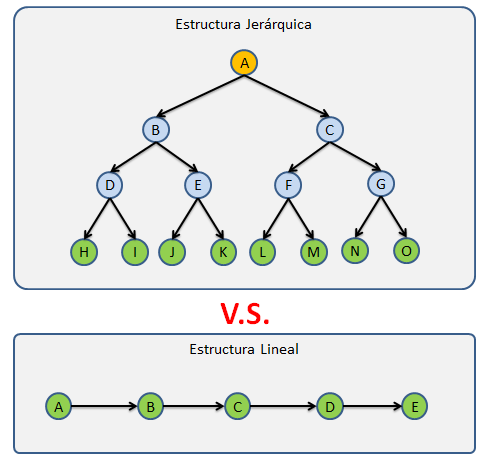
\includegraphics[scale = 0.8]{arbolvslineal.png}
		\caption{Estructura de un \'arbol vs estructura lineal}
		\label{fig:arbol}
	\end{figure}
	
	De esta forma, podemos enumerar los siguientes elementos que conforman un \'arbol \cite{estructuraarboles}:
	\begin{itemize}
		\item \textbf{Nodos:} Se le llama nodo a cada elemento que contiene un \'arbol.
		\item \textbf{Nodo ra\'iz:} Se llama nodo ra\'iz o simplemente ra\'iz al primer nodo de un \'arbol. Solo un nodo del \'arbol puede ser la ra\'iz.
		\item \textbf{Nodo padre:} Se llaman as\'i a aquellos nodos que tienen al menos un hijo.
		\item \textbf{Nodo hijo:} Son aquellos nodos que tienen un padre.
		\item \textbf{Nodo hermano:} Los nodos hermanos son aquellos nodos que comparten un mismo padre.
		\item \textbf{Nodo hoja:} Son todos los nodos que no tienen hijos, los cuales siempre se encuentran en los extremos del \'arbol.
		\item \textbf{Nodo rama o internos:} Estos son todos aquellos nodos que no son la ra\'iz  y que ademas tiene al menos un hijo.
	\end{itemize}
	
	\begin{figure}[h]
		\centering
		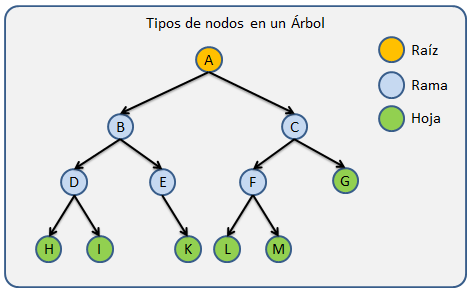
\includegraphics[scale = 0.8]{tiposdenodos.png}
		\caption{Tipos de nodos}
		\label{fig:nodos}
	\end{figure}
	
	\begin{figure}[h]
		\centering
		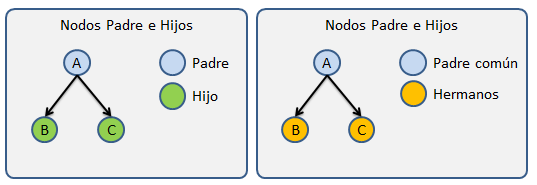
\includegraphics[scale = 0.8]{nodospadrehijohermano.png}
		\caption{Nodos padre, hijos y hermanos}
		\label{fig:relacionnodos}
	\end{figure}
	
	Por otra parte, haciendo uso de estos elementos, definimos los siguientes conceptos o caracter\'isticas sobre un \'arbol:
	
	\begin{itemize}
		\item \textbf{Nivel:} Nos referimos como nivel a cada generaci\'on dentro del \'arbol. Por ejemplo, cuando a un nodo hoja le agregamos un hijo, el nodo hoja pasa a ser un nodo rama pero, adem\'as, el \'arbol crece una generaci\'on por lo que tiene un nivel m\'as.Cada generaci\'on tiene un nivel distinto que el resto de generaciones. De este modo: 
		\begin{enumerate}
			\item Un \'arbol vac\'io tiene 0 niveles.
			\item El nivel del nodo ra\'iz es 1
			\item El nivel de cada nodo se calcula contando cuantos nodos existen sobre \'el hasta llegar a la ra�z m\'as 1. Tambi\'en podr\'a calcularse de forma inversa, es decir, contando cuantos nodos existen desde la ra\'iz hasta el nodo buscado m\'as 1.
		\end{enumerate}
		\item \textbf{Altura:} Llamamos altura al n\'umero m\'aximo de niveles de un \'arbol. Teniendo en cuenta esta idea, podemos calcular tambi\'en la altura de cada nodo como la altura del sub\'arbol correspondiente a ese nodo. Se calcula de manera recursiva de la siguiente manera:
		$$ altura = max(altura(hijo1), altura(hijo2), ..., altura(hijoN)) + 1 $$
		\begin{figure}[h]
			\centering
			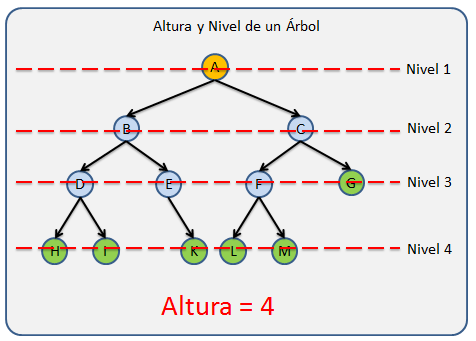
\includegraphics[scale = 0.8]{alturaniveles.png}
			\caption{Niveles y altura de un \'arbol}
			\label{fig:nivelyaltura}
		\end{figure}
		\item \textbf{Peso:} Llamamos peso al n\'umero de nodos que tiene un \'arbol. Este factor nos da una idea del tama\~{n}o del \'arbol y el tama\~{n}o en memoria que nos puede ocupar en tiempo de ejecuci\'on. Se puede calcular mediante cualquier algoritmo que recorra todos los nodos del \'arbol. De forma recursiva, el peso se puede calcular como la suma del peso de los sub\'arboles hijos m\'as 1:
		$$ peso = peso(hijo1) + peso(hijo2) + ... + peso(hijoN) + 1$$
		\item \textbf{Orden:} Es es el n\'umero m\'aximo de hijos que puede tener un nodo.
		\item \textbf{Grado:} N\'umero mayor de hijos que tiene alguno de los nodos del \'arbol. Observemos que el grado se encuentra limitado por el orden. Para calcularlo, al igual que en los casos anteriores, lo hacemos de forma recursiva contando el n\'umero de hijos de cada sub\'arbol y el del nodo actual:
		$$ grado = max(grado(hijo1), grado(hijo2), ..., grado(hijoN), grado(this))$$
	\end{itemize}
	
	Podemos encontrar distintas clasificaciones para los \'arboles, pero para el prop\'osito de este trabajo s\'olo mencionaremos una, dentro de la cual se encuentra el tipo de \'arboles con los que trabajaremos en el resto de la secci\'on.
	\\
	
	Dicho tipo de \'arboles son los conocidos como \textit{\'arboles n-arios}. Los \'arboles n-arios son aquellos \'arboles donde el n\'umero m\'aximo de hijos por nodo es \textit{n}. En particular, los \'arboles cuyo n\'umero m\'aximo de hijos por nodos es 2 reciben el nombre de \textit{\'arboles binarios}. Obs\'ervese que los \'arboles binarios tienen grado 2.
	\\
	
	Definimos entonces los \textbf{\'arboles binarios balanceados}, \textbf{\'arboles binarios de b\'usqueda balanceados}, o simplemente, \textbf{\'arboles AVL} \cite{arbolAVL} como aquellos \'arboles binarios en los que las alturas de los dos sub\'arboles de cada nodo difieren, a lo sumo, en 1. Reciben este nombre en honor a sus creadores Adelson-Velski y Landis \cite{Adelson-Velsky} y es la estructura de datos que usaremos a lo largo de esta secci\'on para mejorar algunos de los m\'etodos voraces que vimos con anterioridad.
	\\
	
	Sobre este tipo de \'arboles definimos el \textit{factor de equilibrio} (FE), que no es m\'as que la diferencia entre las alturas de sus sub\'arboles, es decir:
	
	$$ FB = altura(hijoDrch) - altura(hijoIzq) $$
	
	De este modo, deducimos que los posibles valores para el FE son -1, 0 y 1. Que un nodo tenga un FE igual a 0 indicar\'a que las alturas del hijo derecho y el izquierdo son iguales. Por otro lado, que el FE sea 1 significa que la altura del hijo derecho es mayor que la del izquierdo, mientras que cuando vale -1 tenemos el caso contrario, es decir, que la altura del hijo izquierdo es mayor a la del hijo derecho.
	\\
	
	En caso de que el \'arbol no est\'e balanceado, es decir, que se desequilibre a medida que vamos introduciendo nuevos nodos, habr\'a que rebalancear el \'arbol para que siga siendo un \'arbol AVL v\'alido.
	\\
	
	\begin{figure}[h]
		\centering
		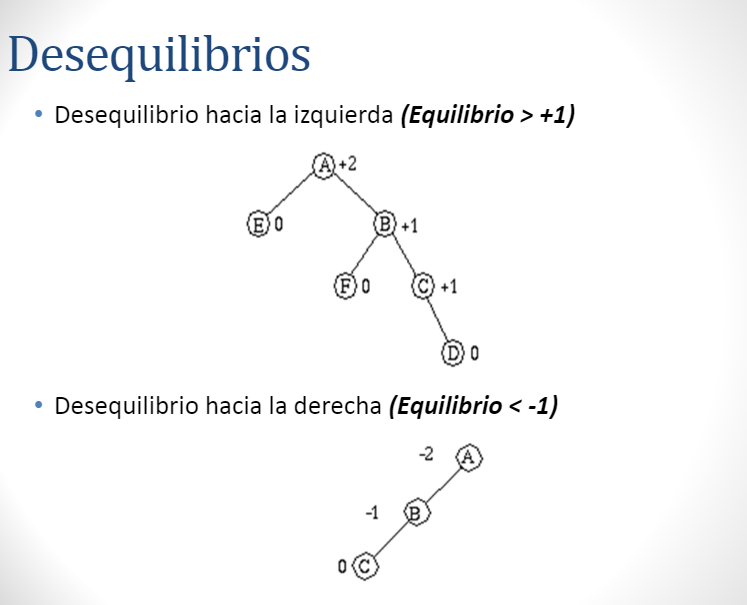
\includegraphics[scale = 0.8]{desequilibrios.png}
		\caption{Tipos de desequilibrios}
		\label{fig:desequilibrio}
	\end{figure}
	
	Por consiguiente, en el caso de que el \'arbol est\'e desequilibrado, existen cuatro operaciones que corrigen el balanceo \cite{arbolesAVL}. A saber: 
	
	\begin{enumerate}
		\item Rotaci\'on simple a la derecha.
		
		\begin{figure}[h]
			\centering
			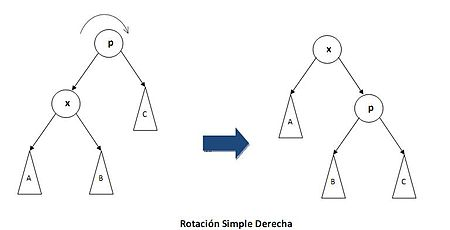
\includegraphics[scale = 1.2]{RotSimDrcha.png}
			\caption{Rotaci\'on simple a la derecha.}
			\label{fig:rotSimpleDrcha}
		\end{figure}
		
		\item Rotaci\'on simple a la izquierda.
		
		\begin{figure}[h]
			\centering
			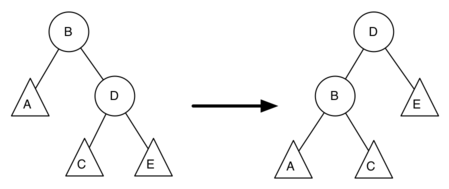
\includegraphics[scale = 1.5]{RotSimIzq.png}
			\caption{Rotaci\'on simple a la izquierda}
			\label{fig:rotSimpleIzq}
		\end{figure}
		
		\item Rotaci\'on doble a la derecha.
		\item Rotaci\'on doble a la izquierda.
	\end{enumerate}
	
	Las rotaciones dobles son, b\'asicamente, realizar dos rotaciones simples seguidas. De esta forma, un rotaci\'on doble a la derecha es una rotaci\'on simple a la derecha seguida de una rotaci\'on simple a la izquierda. Por otro lado, una rotaci\'on doble a la izquierda se compone de una rotaci\'on simple a la izquierda seguida de una rotaci\'on simple a la derecha.
	\\
	
	As\'i, por ejemplo, una rotaci\'on doble a la derecha resultar\'ia como en la Figura \ref{fig:rotDobDrcha}.
	\pagebreak{}
	
	\begin{figure}[h]
		\centering
		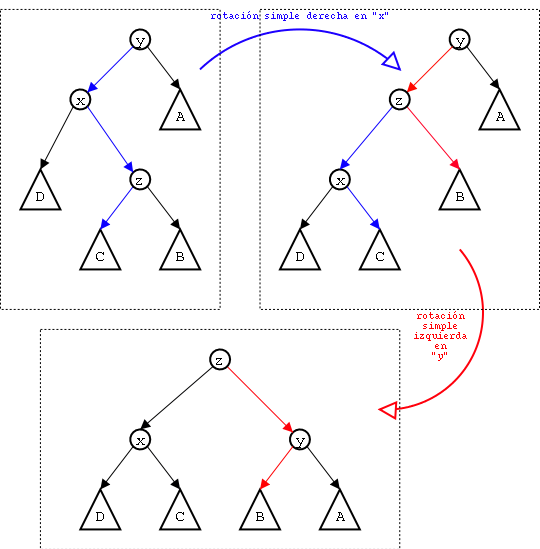
\includegraphics[scale = 0.7]{RotDobDrcha.png}
		\caption{Rotaci\'on doble a la derecha}
		\label{fig:rotDobDrcha}
	\end{figure}
	
	Como vemos, la idea detr\'as de estas operaciones de equilibrado, es desplazar los nodos de la rama m\'as larga a la rama m\'as corta. Debemos mencionar que existen m\'as tipos de equilibrados y que del que estamos haciendo uso es el que se conoce como equilibrado en altura. Una caracter\'istica importante de este tipo de equilibrado es que se hace en orden ascendente, es decir, s\'olo en el camino desde el nodo insertado o borrado hacia la ra\'iz.
	\\
	
	Hasta ahora hemos dado definido el tipo de \'arbol que vamos a usar y, sobre \'el, hemos definido una serie de conceptos entre los cuales el m\'as importante hasta ahora ha sido el de equilibrio. Por otra parte, para garantizar este equilibrio, hemos definido las operaciones de las rotaciones. Por lo tanto, la pregunta que nos hacemos a continuaci\'on de manera natural es: ?`por qu\'e estamos interesados en utilizar esta estructura de datos?
	\\
	
	Y la respuesta la encontramos en la soluci\'on de la cuesti\'on: ?`cu\'al es la complejidad de la operaci\'on de b\'usqueda en un \'arbol AVL? Ve\'amoslo.
	\\
	
	Supongamos que tenemos un \'arbol AVL de \textit{n} elementos y con una altura \textit{h}. Si queremos buscar un elemento en el \'arbol en el peor de los casos haremos \textit{h} comparaciones. Esto es as\'i porque, en este tipo de \'arboles, tenemos definido un \textit{orden} seg\'un el cual cada nodo padre es "mayor" o "igual" que todos los que est\'as en su hijo izquierdo y "menor" que todos los del hijo derecho.
	\\
	
	\begin{figure}[h]
		\centering
		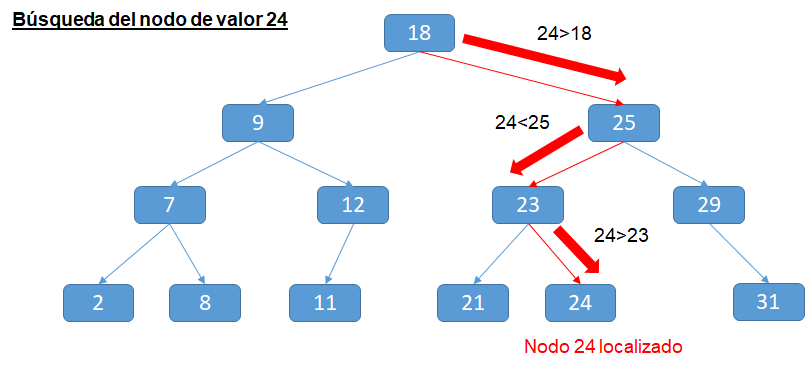
\includegraphics[scale = 0.9]{busquedaarbolpng.png}
		\caption{Ejemplo de b\'usqueda en un \'arbol binario.}
		\label{fig:busquedaAVL}
	\end{figure}
	
	Por lo tanto, la complejidad para localizar un elemento ser\'a \textit{O(h)} \cite{Tema4}. Notemos tambi\'en que, en cada iteraci\'on de la b\'usqueda, dividimos el espacio de b\'usqueda a la mitad. As\'i
	\\
	
	Sea \textit{N(h)} el m\'inimo n\'umero de nodos de un \'arbol AVL de altura h. Entonces 
	
	$$N(h) = 1 + N(h-1) + N(h-2),\hspace{2pt} h > 2,$$
	
	donde el primer sumando se debe al nodo que se encuentra en la ra\'iz del \'arbol, el segundo a que la altura de un hijo debe ser $h-1$ y el tercero a que la diferencia de las alturas de los hijos debe ser menor o igual que 1, y el m\'inimo de nodos corresponde a $h-2$. Por lo tanto,
	
	$$N(h) = O(\phi^{h}) \rightarrow h = O(\log_{\phi}(n))$$
	
	De esta forma vemos que la complejidad de la operaci\'on de b\'usqueda en un \'arbol AVL es $O(h) = O(\log_{\phi}(n))$
	\\
	
	As\'i, las mejoras que vamos a incorporar en esta secci\'on para mejorar algunos de los algoritmos anteriores, no es m\'as que representar la soluci\'on de nuestro problema mediante una estructura de \'arbol AVL en lugar de en una lista (array) de cubos. 
	\\
	
	Los algoritmos que implementaremos haciendo uso de esta estructura ser\'an First Fit, Best Fit, Worst Fit y sus correspondientes algoritmos de tipo decreasing, ya que la implementaci\'on de estos \'ultimos no requiere de gran esfuerzo extra para realizarlos. 
	\\
	
	De nuevo, recordemos que la complejidad de estos algoritmos es $O(n^{2})$ debido a que, a la hora de buscar un cubo donde introducir un nuevo elemento y reordenar el array soluci\'on, estas operaciones resultaban tener una complejidad \textit{O(n)}, por lo que al tener \textit{n} elementos a introducir en los cubos la complejidad de los algoritmos finalmente es $O(n^{2})$. En cambio, como veremos a medida que vayamos realizando los pseudoc\'odigos de los m\'etodos que implementan estos algoritmos, dado que la b\'usqueda en \'arboles AVL tiene complejidad $O(\log_{\phi}(n))$, los algoritmos tendr\'an ahora una complejidad $O(n\log_{\phi}(n))$, lo cual mejora en gran medida la eficiencia de dichos algoritmos a la hora de resolver instancias del BPP muy grandes.
	\\
	
	A continuaci\'on, vamos a estudiar cu\'al es la l\'ogica que siguen estos algoritmos cuando hacen uso de esta estructura de datos. Presentaremos el pseudoc\'odigo de los m\'etodos principales mientras que dejaremos para el cap\'itulo siguiente una explicaci\'on m\'as exhaustiva de c\'omo se ha implementado todo el proyecto.
	
	\subsubsection{First Fit usando \'arboles AVL}
	Dado que un \'arbol est\'a formado por nodos, lo primero que tenemos que establecer es qu\'e informaci\'on va a almacenar cada nodo del \'arbol. De este modo, cada nodo contiene:
	\begin{enumerate}
		\item La altura del nodo en el \'arbol.
		\item La capacidad restante m\'axima del nodo, es decir, la mayor capacidad restante entre la del cubo del nodo actual y la de los cubos de sus dos hijos.
		\item Un cubo, que a su vez contiene:
		\begin{itemize}
			\item Su capacidad restante.
			\item Una lista con los pesos que ya se han introducido.
		\end{itemize}
		\item Aparte de estos datos, cada nodo tambi\'en tendr\'a una referencia a su hijo izquierdo y a su hijo derecho, pero esta informaci\'on solo resulta relevante a la hora de implementar el algoritmo en el ordenador.
	\end{enumerate}
	
	Notemos que, del punto 2, deducimos que la capacidad restante m\'axima del \'arbol ser\'a la capacidad restante m\'axima de la ra\'iz. Adem\'as, si cuando queremos introducir un nuevo objeto en el \'arbol vemos que tiene un peso mayor que la capacidad restante m\'axima de la ra\'iz, esto quiere decir que el objeto no cabe en ninguno de los cubos del \'arbol, es decir, de la soluci\'on, con lo que tendremos que crear un nuevo cubo para este objeto.
	\\
	
	Recordemos que anteriormente tambi\'en mencionamos que sobre los \'arboles AVL tenemos que definir un orden, pero al igual que en la primera implementaci\'on de este algoritmo, el orden que definimos en el \'arbol no es m\'as que el orden en el que se han ido creando los cubos. De esta forma, deducimos que cada vez que creemos un nuevo cubo lo haremos a\~{n}adiendo un nuevo nodo con dicho cubo al final de la \textit{espina derecha}, que no es m\'as que el camino que resulta de recorrer el \'arbol desde la ra\'iz a trav\'es de todos sus hijos derechos, hasta llegar a la hoja que se encuentra en el extremo inferior derecho.
	\\
	
	Observemos que, como siempre introduciremos los nodos nuevos al final de la espina derecha, para equilibrar el \'arbol cuando sea necesario solo har\'a falta realizar rotaciones a la izquierda.
	\\
	
	De esta forma, los m\'etodos que resuelven el algoritmo First Fit haciendo uso de la estructura de \'arboles AVL son los siguientes:
	
	\begin{itemize}
		\item \textbf{addNewBin(bin: Bin)}: Este m\'etodo toma un cubo y lo a\~{n}ade al final de la espina derecha. Para mantener el invariante de los \'arboles AVL, en cada nodo de la espina derecha, si la altura resultante del hijo derecho es m\'as de una unidad superior a la del hijo izquierdo, habr\'a que aplicar una rotaci\'on simple a la izquierda.
		\\
		
		As\'i, el pseudoc\'odigo del m\'etodo ser\'ia
		
		\noindent\fbox{
			\begin{minipage}{\textwidth}
				\begin{algorithmic}
					
					\State{def addNewBin(bin: Bin): Unit}
					\State{//addBinToNode es un m\'etodo recursivo con el que vamos recorriendo cada hijo derecho}
					\State{//hasta llegar al final de la espina derecha, que es donde creamos un nuevo nodo con}
					\State{//el cubo dado}
					\State{def addBinToNode(node: Node): Node}
					\If{(node.right es null)}
					\State{//Esto quiere decir que node no tiene hijo derecho}
					\State{Creamos el nodo hijo derecho de node y a\~{n}adimos el cubo}
					\State{Recalculamos la altura de node}
					\State{Recalculamos la capacidad restante m\'axima de node}
					\State{Devolvemos el nodo node}
					\Else
					\State{//Esto quiere decir que el hijo derecho de node existe y que, por tanto, no estamos}
					\State{//al final de la espina derecha}
					\State{node.right = addBinToNode(node.right)}
					\If{height(node.right) - height(node.left) $>$ 1}
					\State{Hacemos una rotaci\'on simple a la izquierda de node}
					\Else
					\State{Recalculamos la altura de node}
					\State{Recalculamos la capacidad restante m\'axima de node}
					\State{Devolvemos el nodo node}
					\EndIf
					\EndIf
					\If{root es null}
					\State{//Esto quiere decir que el \'arbol est\'a vac\'io}
					\State{Creamos el nodo ra\'iz y le a\~{n}adimos el cubo}
					\Else
					\State{root = addBinToNode(root)}
					\EndIf
					
				\end{algorithmic}
			\end{minipage}
		}
		\\\\
		
		\item \textbf{addFirst(initialCapacity: Int, weight: Int): Unit}: Este m\'etodo toma la capacidad de los cubos del problema, el peso de un objeto a introducir y lo a\~{n}ade al primer cubo que pueda contenerlo o a\~{n}ade un nuevo cubo al final de la espina derecha si el objeto nuevo no cabe en ning\'un cubo. El algoritmo funcionar\'ia de la siguiente forma:
		\begin{itemize}
			\item Si el \'arbol est\'a vac\'io o el objeto no cabe en ning\'un cubo, se a\~{n}adir\'a un nuevo nodo con un cubo con el objeto al final de la espina derecha.
			\item  En otro caso, si la capacidad restante m\'axima del hijo izquierdo es mayor o igual al peso del objeto, se a\~{n}adir\'a el objeto al primer cubo posible del hijo izquierdo.
			\item En otro caso, si la capacidad restante del cubo en el nodo ra\'iz (o nodo padre) es mayor o igual al peso del objeto, se a\~{n}adir\'a el objeto al cubo en la ra\'iz.
			\item En otro caso, se a\~{n}adir\'a el objeto al primer cubo posible del hijo derecho.
		\end{itemize}
		\item \textbf{addAll(): Unit}: Con este m\'etodo a\~{n}adimos todos los objetos de la lista de objetos dada en la instancia del problema y los a\~{n}adimos al \'arbol. Es un m\'etodo muy sencillo cuyo pseudoc\'odigo es
		
		\noindent\fbox{
			\begin{minipage}{\textwidth}
				\begin{algorithmic}
					
					\State{def addAll(): Unit}
					\State{//instance es un objeto que representa una instancia del problema del BP}
					\State{//El objeto instance tiene dos atributos, capacity e items, que son la capacidad de los}
					\State{//cubos y la lista de objetos a introducir en los cubos}
					\For{(item $\leftarrow$ instance.items)}
					\State{addFirst(instance.capacity, item)}
					\EndFor
					
				\end{algorithmic}
			\end{minipage}
		}
		\\\\
	\end{itemize}
	
	Para el estudio de la complejidad, supongamos que tenemos \textit{n} elementos a introducir en los cubos. Dado un elemento nuevo a introducir, en el peor de los casos, tendremos que hacerlo al final de la espina derecha o crear un nodo nuevo aqu\'i tambi\'en. En ambos casos, por lo explicado con anterioridad acerca de la complejidad de los algoritmos de b\'usqueda, tenemos que la complejidad de esta parte del algorimo es $O(\log_{\phi}(n))$. Como tenemos \textit{n} elementos, la complejidad del algoritmo First Fit usando \'arboles AVL es $O(n\log_{\phi}(n))$, como ya hab\'iamos mencionado.
	
	\subsubsection{Best Fit y Worst Fit usando \'arboles AVL}
	
	Vamos a englobar estos dos algoritmos en una misma secci\'on dado que su implementaci\'on solo se diferencia en un \'unico m\'etodo.
	\\
	
	En ambos casos, la informaci\'on que almacenaremos en cada nodo ser\'a:
	\begin{enumerate}
		\item La altura del nodo en el \'arbol.
		\item Un cubo, el cual contiene los atributos del caso anterior.
		\item Al igual que en el caso previo, una referencia a su hijo izquierdo y otra a su hijo derecho.
	\end{enumerate}
	
	A diferencia del \'arbol que construimos para First Fit, en este tenemos que definir un orden diferente, el cual viene dado por la capacidad restante del cubo que hay en cada nodo. Esto es, por ejemplo, un nodo es menor que otro si la capacidad restante del cubo del primer nodo es menor que la capacidad restante del cubo del segundo nodo. 
	\\
	
	Otra diferencia con respecto al algoritmo First Fit es c\'omo introducimos un nuevo elemento. En un principio usamos el mismo criterio que usan los m\'etodos Best Fit y Worst Fit ya definidos. Por ejemplo, para el nuevo m\'etodo Best Fit, si queremos introducir un nuevo elemento en alguno de los cubos de los nodos del \'arbol (si es que es posible), tendremos que buscar aquel nodo cuya capacidad restante del cubo sea la menor de todas aquellas que sean mayores o iguales que el peso del elemento dado. An\'alogamente para el m\'etodo Worst Fit. La peculiaridad se encuentra en c\'omo hacemos esa inserci\'on una vez localizado el cubo, porque recordemos que luego tendremos que reordenar los nodos del \'arbol.
	\\
	
	Y es que, lo que hacemos, es guardar el cubo del nodo localizado con el nuevo elemento a\~{n}adido, borrar dicho nodo y hacer una inserci\'on ordenada del cubo anterior, lo cual se traducir\'a en crear un nuevo nodo en la posici\'on que le corresponda dentro del \'arbol que contenga a dicho cubo.
	\\
	
	Observemos tambi\'en que esto \'ultimo significa que, a diferencia del First Fit en el que solo es necesario hacer rotaciones a la izquierda, aqu\'i tendremos que hacer rotaciones simples tanto a la izquierda como a la derecha. Para ello, como veremos en el cap\'itulo siguiente, implementaremos un m\'etodo general que realice el balanceo del \'arbol haciendo uso de los m\'etodos que se encarguen de hacer las rotaciones simples a la derecha o a la izquierda.
	\\
	
	De este modo, los algoritmos Best First y Worst Fit comparten los siguientes m\'etodos:
	
	\begin{enumerate}
		\item \textbf{insert(bin: Bin): Unit}: Con este m\'etodo creamos un nuevo nodo dentro del \'arbol que contenga al cubo que le indicamos. El pseudoc\'odigo es el siguiente:
		\\
		
		\noindent\fbox{
			\begin{minipage}{\textwidth}
				\begin{algorithmic}
					
					\State{def insert(bin: Bin): Unit}
					\State{//insertRec es un m\'etodo recursivo con el que recorremos los nodos del \'arbol en orden}
					\State{//para encontrar el nodo en cuyo hijo crearemos el nodo nuevo con el cubo}
					\State{def insertRec(node: Node): Node}
					\If{node es null}
					\State{//Esto quiere decir que el nodo en el que nos encontramos est\'a vac\'io y solo ocurrir\'a}
					\State{//cuando lleguemos a la posici\'on donde tenemos que crear el nuevo nodo}
					\State{Creamos el nuevo nodo con el cubo bin introducido}
					\Else
					\State{//getLeftCapacity es un m\'etodo que nos devuelve la capacidad restante de un cubo}
					\State{cmp = bin.getLeftCapacity - node.bin.getLeftCapacity}
					\If{(cmp $<$ 0)}
					\State{//Esta condici\'on significa que la capacidad restante del cubo a introducir es}
					\State{//menor que la capacidad restante del cubo del nodo actual}
					\State{//Entonces compruebo el hijo izquierdo}
					\State{node.left = insertRec(node.left)}
					\Else
					\State{//La capacidad restante del cubo a introducir es mayor o igual que la del cubo}
					\State{//del nodo actual}
					\State{//Compruebo entonces el hijo derecho}
					\State{node.rigth = insertRec(node.right)}
					\EndIf
					\State{//El m\'etodo balance realiza el balanceo del \'arbol, haciendo las rotaciones y}
					\State{//reajustando las alturas de los nodos}
					\State{node.balance}
					\EndIf
					\State{//Empezamos comprobando si podemos insertar el cubo desde la ra\'iz}
					\State{root = insertRec(root)}
				\end{algorithmic}
			\end{minipage}
		}
		\\\\
		
		\item \textbf{add(initialCapacity: Int, weight: Int): Unit}: Dada la capacidad de los cubos y el peso de un objeto a introducir en los mismos, este m\'etodo es el que se encarga de introducirlo en un cubo de alg\'un nodo del \'arbol. Su funcionamiento ya la describimos cuando se explic\'o c\'omo se introduc\'ia un nuevo elemento en el \'arbol. Esto es, primero comprobamos si el elemento cabe en el cubo que almacena alg\'un nodo. Si no cabe en ninguno, creo un nuevo cubo al que le a\~{n}ado el elemento e inserto este cubo en el \'arbol haciendo una llamada al m\'etodo anterior pas\'andole como par\'ametro este cubo. Si cabe en alguno, copio ese cubo, introduzco el elemento y borro el nodo para, a continuaci\'on, llamar de nuevo al m\'etodo anterior pas\'andole como par\'ametro este cubo.
		\\
		
		As\'i el pseudoc\'odigo ser\'ia:
		
		\noindent\fbox{
			\begin{minipage}{\textwidth}
				\begin{algorithmic}
					
					\State{def addl(initialCapacity: Int, weight: Int): Unit}
					\State{//auxBin es una variable auxiliar que me guarda el cubo en el que cabe el elemento si}
					\State{//lo encuentra o un valor None}
					\State{auxBin: Option[Bin] = delete(weight)}
					\If{(auxBin est\'a vac\'io)}
					\State{//Creo un cubo con la capacidad inicial dada}
					\State{bin = new Bin(initialCapacity)}
					\State{A\~{n}ado el peso del elemento al cubo}
					\State{insert(bin)}
					\Else
					\State{Le a\~{n}ado el elemento al cubo que hemos copiado y cuyo nodo hemos borrado}
					\State{Insertamos de nuevo el cubo en el \'arbol}
					\EndIf
					
				\end{algorithmic}
			\end{minipage}
		}
		\\\\
		\item \textbf{addAll(): Unit}: Este m\'etodo es exactamente el mismo que el implementado en First Fit, ya que su \'unica funci\'on es, dada una instancia del problema, ir recorriendo la lista de objetos a introducir en la instancia para a\~{n}adirlos en cubos con la capacidad dada.
	\end{enumerate}
	
	Notemos que en estos m\'etodos ya hemos usado indirectamente a aquel que hace que el m\'etodo Best Fit y Worst Fit sean diferentes, que es la funci\'on que borra los nodos que contienen los cubos en donde vamos a introducir un nuevo elemento (m\'etodo delete que hemos usado en la funci\'on add anterior). Esto es as\'i porque estos m\'etodos incorporan los algoritmos de b\'usqueda de los que hacen uso Best Fit y Worst Fit. 
	\\
	
	\textbf{NO SE SI AQUI DEBERIA EXPLICAR LOS DOS METODOS DELETE JUNTO CON SU PSEUDOCODIGO O DEJARLOS PARA EL CAPITULO SIGUIENTE}
	
	\subsection{Algoritmos evolutivos}
	Los algoritmos evolutivos son una serie de algoritmos metaheur\'isticos inspirados en el proceso evolutivo. Por lo tanto, la idea detr\'as de ellos es sencilla de comprender: partiendo de una poblaci\'on conocida, obtenemos mediante reproducci\'on y selecci\'on natural un individuo "mejor". A continuaci\'on, este nuevo individuo se incorpora a la poblaci\'on de partida y seguimos obteniendo nuevos individuos mediante los mecanismos anteriores y as\'i, sucesivamente. Evidentemente estos nuevos individuos no tienen por qu\'e ser necesariamente mejores, aunque evidentemente trataremos que as\'i sea. Posteriormente, tendremos que especificar cu\'ales son estos mecanismos que simulan los procesos de reproducci\'on y selecci\'on.
	\\
	
	\textbf{MENCIONAR TFG VIGO}
	\\
	
	De esta forma, el algoritmo evolutivo funcionar\'ia como describimos a continuaci\'on:
	
	\begin{enumerate}
		\setcounter{enumi}{-1}
		\item Antes de arrancar propiamente el algoritmo evolutivo, tenemos que hacer un paso previo que se corresponde con la generaci\'on de la poblaci\'on a partir de la cual vamos a ir consiguiendo las posteriores generaciones de individuos (o poblaciones). Esta poblaci\'on tiene un tama\~{n}o prefijado y se encuentra ordenada de mejor a peor, como veremos m\'as adelante.
		\item \textbf{Fase de selecci\'on}. Aqu\'i entramos en el ciclo del algoritmo evolutivo. Aparte de los criterios que establezcamos para que se vayan repitiendo el ciclo, deberemos fijar un tiempo de parada para que el algoritmo finalice una vez se haya alcanzado ese tiempo. Existen diversos m\'etodos de selecci\'on, como el m\'etodo de la ruleta, el m\'etodo de la ruleta extendido con rangos o el m\'etodo de selecci\'on por torneo. Precisamente ser\'a este \'ultimo el que usaremos para implementar nuestro algoritmo evolutivo. Ser\'a mediante estos m\'etodos con los que elegiremos los padres a partir de los cuales obtendremos los nuevos individuos que iremos incorporando a la poblaci\'on.
		\item \textbf{Fase de cruce}. Tanto esta fase como la siguiente, al igual que ocurre en la naturaleza, son dos procesos que no necesariamente tienen que ocurrir, sino que dependen de una cierta probabilidad prefijada. En el caso de que ocurra, lo que el algoritmo realiza es un cruce entre los padres que hemos obtenidos en la selecci\'on anterior para obtener nuevos individuos. Como operaciones de cruce podemos mencionar el cruce de un punto, cruce en dos puntos, cruce uniforme, cruce aritm\'etico, cruce c\'iclico, el cruce PMX.
		\item \textbf{Fase de mutaci\'on}. Con una cierta probabilidad, los nuevos individuos se someten a alteraciones en su \textit{genoma} seg\'un alg\'un patr\'on. Como operaciones de mutaci\'on, podemos citar la mutaci\'on por intercambio repetido (que es la que usaremos) o la mutaci\'on uniforme.
		\item \textbf{Fase de ordenaci\'on}. Recordemos que la poblaci\'on tiene un tama\~{n}o prefijado. Por tanto, en esta fase lo que haremos ser\'a evaluar las soluciones que nos proporcionan estos nuevos individuos generados en la iteraci\'on actual del algoritmo y sustituir los peores individuos de la poblaci\'on por estos nuevos, de manera que el tama\~{n}o de la poblaci\'on siempre sea el mismo y sus individuos se est\'en actualizando en cada iteraci\'on.
		\item Terminamos la iteraci\'on y volvemos a la fase 1.
	\end{enumerate}
	
	Para que el algoritmo quede completamente determinado, aparte de los m\'etodos y variables ya mencionados, tendremos que prefijar el tama\~{n}o de la poblaci\'on, el m\'etodo con el que evaluaremos c\'omo de bueno es un individuo, las probabilidades de cruce y de mutaci\'on y una fuente de aleatoriedad.
	\\
	
	En los algoritmos que hemos visto hasta ahora, dada una instancia del problema de BP, constru\'iamos una soluci\'on introduciendo cada elemento de la instancia seg\'un las reglas que vienen dadas por los algoritmos. As\'i, las mejoras que hemos ido proponiendo, ten\'ian la finalidad de reducir la complejidad de los algoritmos, pero no mejoraban propiamente la soluci\'on. Es decir, por ejemplo, el algoritmo First Fit que usa la implementaci\'on de \'arboles AVL proporciona, en esencia, la "misma" soluci\'on que el primer algoritmo First Fit, con lo que aunque hayamos mejorado su eficiencia, no hemos mejorado mucho su optimalidad.
	\\
	
	El algoritmo evolutivo pretende compensar este hecho. En nuestro caso, el tipo de algoritmo que implementaremos no constituir\'a una mejora en cuanto a la eficiencia de los algoritmos anteriores puesto que, de hecho, fijaremos un tiempo durante el cual el algoritmo se est\'e ejecutando. Tiempo que no tiene por qu\'e ser necesariamente menor del que necesitan os algoritmos anteriores para ejecutarse. En cambio, s\'i que supondr\'a una mejora en cuanto a la calidad de las soluciones.
	\\
	
	Para ello, los individuos que formar\'an la poblaci\'on y aquellos nuevos individuos que iremos generando en cada iteraci\'on del algoritmo, no ser\'an m\'as que permutaciones de los elementos de la lista de objetos dada en una instancia determinada del problema de BP. Por lo tanto, cada individuo de la poblaci\'on tendr\'a dos atributos, que ser\'an la permutaci\'on correspondiente y el n\'umero de cubos que se obtiene al resolver la instancia del problema mediante el m\'etodo con el que dijimos que evaluar\'iamos la calidad de los individuos, Este m\'etodo ser\'a tambi\'en el que nos permita tener ordenados a los individuos de la poblaci\'on de mejor a peor candidato, ya que esta condici\'on es equivalente a ordenar a los individuos seg\'un el n\'umero de cubos que produce su soluci\'on, de menor a mayor cantidad.
	\\
	
	De forma esquem\'atica, el algoritmo evolutivo seguir\'ia el siguiente diagrama:
	
	\begin{figure}[h]
		\centering
		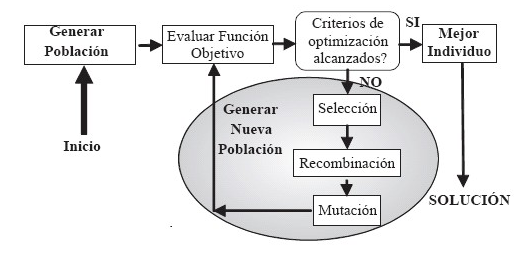
\includegraphics[scale = 0.7]{algev.png}
		\caption{Diagrama de flujo de un algoritmo evolutivo.}
		\label{fig:algEvL}
	\end{figure}
	
	As\'i, el pseudoc\'odigo del algoritmo evolutivo quedar\'ia como:
	
	\noindent\fbox{
		\begin{minipage}{\textwidth}
			\begin{algorithmic}
				
				\State{\textbf{begin}}
				\State{Creamos la poblaci\'on inicial.}
				\State{Evaluamos la poblaci\'on inicial.}
				\State{//La condici\'on de parada del bucle while es que alcancemos la SO o que se agote el tiempo.}
				\While{(no se verifique la condici\'on de parada)}
				\State{Seleccionamos aleatoriamente los padres en la poblaci\'on.}
				\State{Cruzamos con cierta probabilidad a los padres para obtener a los hijos.}
				\State{Mutamos los descendientes con cierta probabilidad.}
				\State{Evaluamos los nuevos individuos generados.}
				\State{Sustituimos los peores individuos de la poblaci\'on por los nuevos individuos que hemos generado.}
				\EndWhile
				
			\end{algorithmic}
		\end{minipage}
	}
	\\\\
	
	
	\chapter{Implementaci\'on}
	
	\section{Introducci\'on}
	En este cap\'itulo vamos a explicar brevemente c\'omo est\'a estructurada la soluci\'on que se propone en este trabajo. En el cap\'itulo anterior hemos explicado los algoritmos que hemos implementado para dar distintas soluciones a un problema de tipo BP por lo que, a continuaci\'on, lo que haremos ser\'a explicar las clases y m\'etodos que hemos implementado para poder llevar a cabo los algoritmos anteriores. En el siguiente enlace podemos consultar el c\'odigo completo:
	\\
	
	\url{https://github.com/RafaelRG94/BinPackingProblem}
	
	\section{Preparaci\'on del problema}
	En esta primera parte vamos a explicar qu\'e clases hemos implementado para introducir los datos y prepararlos para su posterior uso en los algoritmos que hemos presentado previamente.
	
	\subsection{La clase Bin}
	L\'gicamente este es el primer fichero que hemos tenido que implementar. Con \'el hemos creado un objeto con el que representar la informaci\'on que guarda un cubo del problema as\'i como los m\'etodos principales para interactuar con el mismo.
	\\
	
	En primer lugar tenemos dos \'unicos atributos, a saber: \textit{items}, que es un array de tipo buffer y es la variable donde almacenaremos los elementos que se vayan introduciendo en el cubo y \textit{leftCapacity}, que almacena un entero cuya clase recibe como constructor y no es m\'as que la capacidad restante del cubo. El motivo por el que se elige el arraybuffer para almacenar los objetos que se van introduciendo es que es una estructura de datos mutable (que es lo que nos permite ir introduciendo nuevos elemento en el cubo) que comparte mucho de los m\'etodos que los arrays tienen predefinidos. 
	\\
	
	Por otra parte, podemos encontrar los siguientes m\'etodos principales:
	\begin{itemize}
		\item \textbf{add}: Este m\'etodo toma como par\'ametro un entero y lo introduce en el cubo.
		\item \textbf{canAdd}: Dado un entero, esta funci\'on comprueba si el elemento se puede introducir en el cubo.
		\item \textbf{getLeftCapacity}: Con este m\'etodo podemos consultar la capacidad restante de la instancia del cubo que estemos interesados.
	\end{itemize}
	
	\subsection{Las clases ProblemInstance y Solution}
	Estas dos clases las usamos para crear objetos que representen tanto la instancia de un problema de BP como su soluci\'on. Ambos implementan un m\'etodo \textbf{toString} para posteriormente mostrar distintos datos por pantalla. Adem\'as, podemos encontrar los dos siguientes m\'etodos:
	\begin{itemize}
		\item \textbf{sortDescendingInstance}: M\'etodo de la clase ProblemInstance con el que ordenamos de manera descendente la lista de objetos que tenemos en la instancia de un problema BP. Este m\'etodo es necesario para su posterior uso en los algoritmos de tipo decreasing. Su implementaci\'on es muy sencilla dado que lo \'unico que hacemos es copiar la lista de objetos de la instancia del problema, ordenarla y devolver un objeto de tipo ProblemInstance que tenga a esta \'ultima lista como objetos a introducir en los cubos.
		\item \textbf{length}: M\'etodo de la clase Solution con el que devolvemos la longitud de la soluci\'on de una instancia del problema.
	\end{itemize}
	
	\subsection{La clase Utils}
	En el fichero Utils.scala tenemos tres m\'etodos auxiliares de los que posteriormente hacemos uso cuando implementamos los algoritmos:
	
	\begin{itemize}
		\item \textbf{smallerThanTarget}: Se trata de un m\'etodo de b\'usqueda binaria \cite{smallerThanTarget} con el que, dado un entero y un arraybuffer de cubos ordenados seg\'un sus capacidades restantes de forma creciente, encuentra la posici\'on del cubo con la menor capacidad restante que es mayor o igual que el entero dado. 
		\item \textbf{reorderBufferArrays}: Este m\'etodo toma como par\'ametros un arraybuffer de cubos que se encuentran ordenados seg\'un sus capacidades restantes y la posici\'on de un elemento del array que se encuentra desordenado y, lo que realiza, es la reordenaci\'on de dicho elemento. Su implementaci\'on es sencilla dado que, lo que hacemos, es usar el m\'etodo anterior para encontrar la nueva posici\'on de dicho cubo en el array para luego guardar el cubo en una variable auxiliar y, haciendo uso de que los arraybuffer son estructuras de datos mutables, usar los m\'etodos predefinidos de las librer\'ias de Scala para borrar el elemento del array y reinsertarlo en la posici\'on que hab\'iamos calculado previamente.
		\item \textbf{sortDescending}: Este es un m\'etodo de ordenaci\'on que usamos para ordenar de manera descendente los elementos de la lista de objetos que nos proporciona las distintas instancias del problema. B\'asicamente hacemos uso del algoritmo QuickSort para realizar tal ordenaci\'on \cite{sortDescending}.
	\end{itemize}
	
	\section{Algoritmos voraces}
	Esta parte del c\'odigo se corresponde con aquellas clases que implementan los algoritmos de tipo greedy. Recordemos que la mayor\'ia de algoritmos propuestos tienen dos implementaciones diferentes en funci\'on de qu\'e tipo de estructura de datos usemos para almacenar la soluci\'on que vamos calculando. As\'i, tenemos:
	\begin{itemize}
		\item Ficheros de los algoritmos que almacenan sus soluciones en un \textbf{arraybuffer}: . 
		\begin{enumerate}
			\item AlmostWorstFit.
			\item BestFit.
			\item BestFitDecreasing.
			\item FirstFit.
			\item FirstFitDecreasing.
			\item NextFit.
			\item NextKFit.
			\item WorstFit.
			\item WorstFitDecreasing.
		\end{enumerate}
		Estos ficheros contienen los m\'etodos de la clase de los objetos que, dada una instancia del problema de BP, resuelven el problema seg\'un los algoritmos que hemos descrito en la primera parte del segundo cap\'itulo, almacenando cada nuevo cubo que se va creando en las iteraciones en un arraybuffer.
		\item Ficheros de los algoritmos que almacenan sus soluciones en un \textbf{\'arbol AVL}:
		\begin{enumerate}
			\item BFAVLTree.
			\item BFDAVLTree.
			\item FFAVLTree.
			\item FFDAVLTree.
			\item WFAVLTree.
			\item WFDAVLTree.
		\end{enumerate}
		Estos ficheros contienen los m\'etodos necesarios para implementar los algoritmos Best Fit, First Fit, Worst Fit y sus respectivos algoritmos de tipo decreasing almacenando los cubos de la soluci\'on en \'arboles AVL.
	\end{itemize} 
	
	Como ya mencionamos en el cap\'itulo anterior, los m\'etodos necesarios para implementar los algoritmos Best Fit y Worst Fit mediante \'arboles AVL son pr\'acticamente iguales, cambiando \'unicamente el m\'etodo \textbf{delete} de ambos. Por tanto, para tener un c\'odigo m\'as limpio, se ha creado la clase abstracta AVLTree para implementar todos los m\'etodos de los que hacen uso ambos alogirtmos. Posteriormente, las clases BFAVLTree y WFAVLTree heredan de la clase abstracta anterior para implementar el m\'etodo delete.
	\\
	
	\textbf{EXPLICO AQUI LAS DIFERENCIAS DE LOS METODOS DELETE?}
	
	\section{El algoritmo evolutivo}
	Recordemos que el algoritmo evolutivo va realizando iteraciones hasta que alcanza una condici\'on de parada. En nuestro caso, dicha condici\'on de parada es que se est\'e ejecutando durante el tiempo que le indiquemos. Para ello, la primera clase que implementamos es la clase \textbf{Timer}. Dicha clase contiene los m\'etodos necesarios para obtener el tiempo que marca el reloj interno del ordenador y as\'i, poder establecer un instante inicial y ser capaces de medir intervalos de tiempo \cite{Vigo}.
	
	\subsection{Clases para generar la poblaci\'on inicial}
	\subsubsection{Individual}
	Los objetos de esta clase pretenden representar a los individuos que forman a la poblaci\'on. Por otro lado, como el objetivo del algoritmo evolutivo es encontrar la permutaci\'on de la lista de objetos dada en una instancia del problema de BP con la que obtenemos la mejor soluci\'on del problema seg\'un un algoritmo concreto, la informaci\'on que almacenan los objetos de la clase es la permutaci\'on correspondiente de la lista de objetos a introducir en los cubos, el n\'umero de cubos que obtenemos cuando resolvemos el problema seg\'un un algoritmo dado y los m\'etodos necesarios para interactuar con estos datos.
	
	\subsubsection{Populations}
	El fichero \textbf{Populations.scala} contiene un objeto de tipo Populations con los m\'etodos auxiliares necesarios para luego crear distintos tipos de poblaciones. Recordemos que la poblaci\'on del algoritmo evolutivo no solo contiene las distintas permutaciones de la lista de objetos dada en la instancia del problema, sino tambi\'en el n\'umero de cubos que obtenemos cuando resolvemos el problema para las distintas permutaciones seg\'un el m\'etodo que le indicamos para, posteriormente, ordenar esas permutaciones de mejor a peor seg\'un el n\'umero de cubos obtenidos. Por lo tanto, podemos tener distintos algoritmos evolutivos seg\'un el m\'etodo con el que decidamos resolver las distintas instancias que nos porporcionan los individuos de la poblaci\'on.
	\\
	
	En este sentido, en Populations podemos identificar dos partes claramente diferenciadas:
	\begin{itemize}
		\item \textbf{initPopulation}: Con este m\'etodo, dada una instancia del problema de BP y una funci\'on \textit{Solver} (es decir, una funci\'on con la que resolvemos la instancia del problema), generamos una poblaci\'on (que no es m\'as que un array de individuos) para el algoritmo evolutivo. Para ello, lo que hacemos es que vamos generando permutaciones de la lista de objetos de la instancia del problema de BP mediante el algoritmo de Fisher-Yates (funci\'on shuffle), luego resolvemos la permutaci\'on obtenida con el Solver seleccionado y finalmente ordenamos a los individuos de mejor a peor. La caracter\'stica fundamental por la que elegimos el algoritmo de Fisher-Yates es que genera cada permutaci\'on seg\'un una distribuci\'on uniforme.
		\item M\'etodos con los que generamos distintas poblaciones seg\'un los \textit{Solvers} de los que disponemos (indicamos \'unicamente que algoritmo usan para resolver las instancias):
		\begin{enumerate}
			\item \textbf{fFPopulation}: First Fit.
			\item \textbf{bFPopulation}: Best Fit.
			\item \textbf{wFPopulation}: Worst Fit.
			\item \textbf{aWFPopulation}: Almost Worst Fit.
			\item \textbf{fFAVLTreePopulation}: First Fit (seg\'un el esquema de \'arbol AVL).
			\item \textbf{bFAVLTreePopulation}: Best Fit (seg\'un el esquema de \'arbol AVL).
			\item \textbf{wFAVLTreePopulation}: Worst Fit (seg\'un el esquema de \'arbol AVL).
		\end{enumerate} 
	\end{itemize}
	
	A continuaci\'on, vamos a probar lo afirmado sobre el algoritmo de Fisher-Yates \cite{Vigo}
	
	\begin{lema}(Buen funcionamiento del algoritmo Fisher-Yates)\hfill\break
		Sea $v = (v_{1},...,v_{n})$ un vector con $\{v_{i}\}_{i=1}^{n}=\{1,...,n\}$, esto es, sus componentes son los elementos 1,...,n permutados. Sean $i \in \{1,...,n\}$ y $k \in \mathbb{N}^{+}$. Definimos la variable aleatoria $X_{i}^{k}$ como la nueva posici\'on del elemento i-\'esimo despu\'es de la k-\'esima permutaci\'on mediante el algoritmo Fisher-Yates (de izquierda a derecha). Entonces $X_{i}^{k} \sim U(1,...,n)$.
	\end{lema}
	
	\begin{proof}
		Nuestro objetivo es el de determinar que, para todos \textit{i} y \textit{k}, la posibilidad de que el elemento \textit{i}-\'esimo caiga en cualquier casilla sea $\frac{1}{n}$. Vamos a hacerlo por inducci\'on sobre \textit{k}.
		\begin{itemize}
			\item Caso $k=1$. Aprovechamos la recursividad del algoritmo para demostrar que $X_{i}^{k} \sim U(1,...,n)$.
			\\
			
			Para $n = 1$ no hay nada que probar, y para $n = 2$, notamos que el bucle principal tiene una \'unica iteraci\'on. Supuesto que $j_{1}$ puede valer 1 con probabilidad $\frac{1}{2}$ o 2 con probabilidad $\frac{1}{2}$, $X_{1}^{1}, X_{1}^{2} \sim U(1,2)$ como quer\'iamos ver.
			\\
			
			Suponemos ahora que el resultado es cierto para $n$ y veamos que se cumple para $n+1$. Para aprovechar la hip\'otesis de inducci\'on, discriminamos la posici\'on 1 para aplicar dicha hip\'otesis sobre el resto de elementos. Si en la primera iteraci\'on $j_{1} = 1$, entonces $v_{1}$ permanece en la casilla 1. La posici\'on 1 no se ve afectada por las iteraciones siguientes, de manera que $v_{1}$ permanecer\'a en la posici\'on 1 acabada la permutaci\'on. Por el contrario, si en la primera iteraci\'on $j_{1} \neq 1$, al finalizar \'esta el elemento $v_{1}$ se encontrar\'a en una posici\'on distinta de 1, a la que no podr\'a regresar. El valor de $j_{1}$ determina la posici\'on de $v_{1}$. Notamos por $A$ el suceso $"j_{1} = 1"$ Entonces:
			$$P(X_{1}^{1} = 1) = P(A) = \frac{1}{n+1}$$.
			
			Si vemos tambi\'en que, dado $x \neq 1, P(X_{1}^{1} = x) = \frac{1}{n+1}$, habremos acabado la inducci\'on (para $k = 1$). Para que $v_{1}$ acabe en la posici\'on $x$, despu\'es de ser colocado en la posici\'on $j_{1}$ tras la primera iteraci\'on, solo queda que el elemento ahora en posici\'on $j_{1}$ acabe en la casilla $x$, a lo que llamamos suceso $B$. Ahora bien, dejando de lado la primera posici\'on, podemos pensar en el resto del vector como un vector de tama\~{n}o $n$ sobre el que se puede emplear la hip\'otesis de inducci\'on. En tales circunstancias, la probabilidad de que el elemento en posici\'on $j_{1}$ acabe en la posici\'on $x$ es $\frac{1}{n}$.
			$$P(X_{i}^{1} = x) = P(\={A}\cap B) = P(B|\={A})P(\={A}) = \frac{1}{n} \frac{n}{n+1}$$.
			
			\item Caso $k+1$ y supuesto cierto para $k$. Veamos que $X_{i}^{k+1} \sim U(1,...,n)$. Consideremos entonces $m \in \{1,...,n\}$ y veamos que $P(X_{i}^{k+1} = m) = \frac{1}{n}$.
			$$P(X_{i}^{k+1} = m) = \sum_{j=1}^{n} P(X_{j}^{k+1} = m|X_{i}^{k} = j) P(X_{i}^{k} = j) = \sum_{j=1}^{n} \frac{1}{n} \frac{1}{n} = \frac{1}{n}$$.
			
			En la primera igualdad hemos hecho uso del teorema de la probabilidad total y en la segunda de dos cosas: la probabilidad condicionada coincide con la probabilidad asociada a permutar los elementos una vez y puede aplicarse el caso $k = 1$; en la otra probabilidad hemos empleado la hip\'otesis de inducci\'on.
		\end{itemize}
	\end{proof}
	
	\subsubsection{Population}
	El fichero Population.scala consta de una clase abstracta Population que implementa los m\'etodos necesarios a la hora de interactuar con los distintos tipos de poblaciones. Los m\'as importantes:
	\begin{enumerate}
		\item \textbf{binaryTournament}: M\'etodo que implementa el algoritmo del torneo binario con el cual seleccionamos un individuo de la poblaci\'on aleatoriamente.
		\item \textbf{binaryInsertion}: M\'etodo de inserci\'on binaria con el que, dado un nuevo individuo, lo sustituimos por uno de los que se encuentran en la poblaci\'on para insertarlo.
	\end{enumerate}
	
	Adem\'as, dentro del fichero tenemos definidas otras clases que extienden a la clase abstracta anterior y que hacen uso de los m\'etodos del objeto Populations para as\'i definir las distintas poblaciones seg\'un el \textit{Solver} elegido para resolver la instancia del problema de BP.
	
	\subsection{Clases para los cruces y mutaciones}
	Por una parte tenemos la clase \textbf{Crossover}, la cual implementa dos algoritmos de cruce distintos:
	\begin{enumerate}
		\item Algoritmo de cruce seg\'un el esquema PMX (Partially Mapped Crossover): \textbf{pmx}.
		\item Algoritmo de cruce por vectores de inversi\'on: \textbf{inversionCrossover}. Se define como vector de inversiones de una permutaci\'on $(\pi(i))_{i=1}^{n}$ un vector $(a_{i})_{i=1}^{n}$ donde $a_{i}$ indica el n\'umero de elementos situados a la izquierda de $i$ que son mayores que $i$ \cite{Vigo}.
	\end{enumerate}
	Para m\'as informaci\'on acerca de estos esquemas as\'i como del c\'odigo en el que nos hemos basado para desarrollar los algoritmos que usamos, consultar \cite{Vigo}.
	\\
	
	Por otra parte, en la clase \textbf{Mutation} tenemos los siguientes algoritmos para representar una mutaci\'on en los individuos de la poblaci\'on (notemos que cuando hablemos de los \textit{genes} nos referiremos a los elementos de las permutaciones de la lista de objetos de la instancia del problema de BP) \cite{Vigo}:
	\begin{enumerate}
		\item \textbf{swapMutation}: Los genes de los extremos izquierdo y derecho intercambian sus posiciones.
		\item \textbf{insertMutation}: El gen situado en el extremo derecho se coloca yuxtapuesto a la derecha del gen del extremo izquierdo y desplaza a la derecha todos los que se encontraban en la franja central.
		\item \textbf{scrambleMutation}: Se permutan los genes de la franja central.
		\item \textbf{inversionMutation}: Se invierte el orden de los genes de la franja central.
	\end{enumerate}
	
	Finalmente tenemos la clase \textbf{EvolutionaryAlgorithm} la cual, siguiendo el esquema descrito en el cap\'itulo anterior, hace uso de las clases que acabamos de describir y sus m\'etodos para implementar el m\'etodo \textbf{evolve}, el cual resuelve el algoritmo evolutivo.
	
	\chapter{Conclusiones}
	La finalidad de este trabajo es la de, a trav\'es de un problema de optimizaci\'on combinatoria concreto, pasar del marco te\'orico de las matem\'aticas al pr\'actico. Para ello, hemos hecho uso de la potencia de c\'omputo que nos ofrecen los ordenadores, los cuales nos permiten dar mejores soluciones para este tipo de problemas a medida que la tecnolog\'ia avanza. Este hecho ha quedado reflejado, sobre todo, en el algoritmo evolutivo, ya que cuanto m\'as potente sea la m\'aquina de la que disponemos, m\'as iteraciones podremos realizar en el mismo intervalo de tiempo.
	\\
	
	En realidad, todo lo que se ha expuesto a lo largo del trabajo ha sido para concurrir en el algoritmo evolutivo y ver la cantidad de posibilidades que ofrece. Hemos comenzado explicando una de las versiones m\'as simples del problema de empaquetamiento; posteriormente, hemos presentado una serie de algoritmos que siguen el esquema de los m\'etodos voraces para resolverlo, es decir, el de aquellos m\'etodos que no se replantean las decisiones ya tomadas. A su vez, hemos comprobado que cuanto mejor elecci\'on quisieramos hacer a la hora de introducir un elemento en uno de los cubos, los algoritmos resultantes son cada vez menos eficientes.
	\\
	
	A continuaci\'on, hemos conseguido una mejora significativa en las complejidades de los algotirmos anteriores haciendo uso de la estructura de \'arboles AVL para almacenar la soluci\'on de las instancias del problema. Esto implica, a su vez, que la implementaci\'on del algoritmo sea m\'as compleja.
	\\
	
	Una vez hecho todo este trabajo, hemos podido pasar propiamente a la implementaci\'on del algoritmo evolutivo, pues su funcionamiento se basa en cualquiera de los m\'etodos presentados hasta ahora. De esta forma, vemos que podemos tener un algoritmo evolutivo diferente por cada uno de estos m\'etodos. Adem\'as, si tenemos en cuenta los diferentes algoritmos de selecci\'on, de cruce y de mutaci\'on que hay, vemos que podemos encontrar multitud de combinaciones de todos estos m\'etodos que dan distintos algoritmos evolutivos, lo cual pone de manifiesto la cantidad de opciones existentes a la hora de obtener una "buena" soluci\'on de un problema dado en un tiempo "aceptable". 
	\\ 
	
	Como trabajo futuro, queda pendiente el comparar y analizar c\'omo cada uno de estos m\'etodos resuelven distintas instancias cada vez mayores del problema de empaquetamiento para as\'i verificar que, lo que obtenemos, se ajusta a los resultados y conclusiones que aqu\'i se han expuesto.
	
	No obstante, queda tambi\'en claro la necesidad de encontrar mejores algoritmos que nos permitan resolver problemas cuyo espacio de b\'usqueda de soluciones sea muy grande en tiempos razonables y no solo en este tipo de problemas. En general, a medida que la tecnolog\'ia avanza y con ello nuestra capacidad de generar y recopilar datos, se hace m\'as y m\'as necesario que nuestra capacidad de procesar esos datos, analizarlos y obtener conclusiones y resultados a partir de ellos sea cada vez mejor. Es gracias a ello que, al igual que nuestro algoritmo evolutivo, la especie humana consigue adaptarse, mejorar y evolucionar.
	
	\addcontentsline{toc}{chapter}{Bibliograf\'{\i}a}
	\bibliographystyle{plain}
	\bibliography{ref}% Crear archivo bib con referencias en bibtex
	

	
	
\end{document}
